\documentclass[12pt,fleqn]{book} %taille de la police par défaut, et équations jusitifées à gauche
\usepackage[top=3cm,bottom=3cm,left=3.2cm,right=3.2cm,headsep=10pt,a4paper]{geometry} % marges
\usepackage{xcolor}
\definecolor{enstabGreen}{HTML}{C8D200} 	%vert  	#c8d200 
\definecolor{enstabLightGreen}{HTML}{E9ED99} 	%vert  	#c8d200 
\definecolor{enstabLightBlue}{HTML}{009EE0} %bleu clair 	#009ee0
\definecolor{enstabVeryLightBlue}{HTML}{99D8F3} %bleu clair 	#009ee0
\definecolor{enstabDarkBlue}{HTML}{005C8F}	%bleu foncé 	#005c8f
\definecolor{enstabDarkGrey}{HTML}{333333}	%gris fort 	#333333
\definecolor{enstabLightGrey}{RGB}{48,48,48}	%gris fort 	#333333
\definecolor{enstabParme}{HTML}{8878B2}		%parme 	#8878b2
\definecolor{enstabOrange}{HTML}{F18E00} 	%orange 	#f18e00
\usepackage[colorlinks=true,
        urlcolor=enstabLightBlue,
        anchorcolor=enstabDarkBlue,
        linkcolor=enstabDarkBlue,
        citecolor=enstabDarkGrey,
        pdfauthor={Johan B. C. Engelen},
        pdfkeywords={SVG; LaTeX; Inkscape},
        pdftitle={How to include an SVG image in LaTeX},
        pdfsubject={Describes how to include an SVG image easily in LaTeX using Inkscape}] {hyperref}
\usepackage{url}
\usepackage[utf8]{inputenc} % lettres accentuées
\usepackage[T1]{fontenc}    % Use 8-bit encoding that has 256 glyphs
\usepackage[frenchb]{babel} % Pour le français
\usepackage{cclicenses}     % Licences CC
\usepackage{epigraph}
\usepackage{eso-pic}        % pour une image en fond, page de titre
\usepackage{graphicx}       % Pour inclure des images
\graphicspath{{images/}}    % Où sont les images ?

\usepackage{listings}      % Pour coloriser les codes que vous insérez
\lstset{ %
  backgroundcolor=\color{white},   % choose the background color; you must add \usepackage{color} or 
  basicstyle=\footnotesize\ttfamily,        % the size of the fonts that are used for the code
  breakatwhitespace=false,         % sets if automatic breaks should only happen at whitespace
  breaklines=true,                 % sets automatic line breaking
  captionpos=b,                    % sets the caption-position to bottom
  commentstyle=\color{enstabOrange},    % comment style
  deletekeywords={...},            % if you want to delete keywords from the given language
  escapeinside={\%*}{*)},          % if you want to add LaTeX within your code
  extendedchars=true,              % lets you use non-ASCII characters; for 8-bits encodings only, does not work with UTF-8
  %frame=single,                    % adds a frame around the code
  keepspaces=true,                 % keeps spaces in text, useful for keeping indentation of code (possibly needs columns=flexible)
  keywordstyle=\color{enstabDarkBlue},       % keyword style
  %language=Octave,                 % the language of the code
  morekeywords={*,...},            % if you want to add more keywords to the set
  numbers=left,                    % where to put the line-numbers; possible values are (none, left, right)
  numbersep=8pt,                   % how far the line-numbers are from the code
  numberstyle=\tiny\color{enstabDarkGrey}, % the style that is used for the line-numbers
  rulecolor=\color{black},         % if not set, the frame-color may be changed on line-breaks within not-black text (e.g. comments (green here))
  showspaces=false,                % show spaces everywhere adding particular underscores; it overrides 'showstringspaces'
  showstringspaces=false,          % underline spaces within strings only
  showtabs=false,                  % show tabs within strings adding particular underscores
  stepnumber=5,                    % the step between two line-numbers. If it's 1, each line will be numbered
  stringstyle=\color{enstabParme},     % string literal style
  tabsize=2,                       % sets default tabsize to 2 spaces
  title=\lstname                   % show the filename of files included with \lstinputlisting; also try caption instead of title
}
\usepackage{subcaption}




\usepackage{booktabs}       % pour de jolis tableaux
%\usepackage{fancyhdr}       % pour des entêtes et pieds de pages améliorés.
\usepackage{makeidx}        % requis pour faire les index
\usepackage{glossaries} %requis pour faire le glossaire
     % Ce fichier contient tous les packages nécessaires à la compilation
\makeindex           % donne l'ordre de créer l'index
\newacronym{IS}{IS}{Ingénierie Système}
\newacronym{WBS}{WBS}{Work Breakdown Structure}  % ce fichier contient les entrées du glossaire
\makeglossaries      % donne l'ordre de créer le glossaire

\begin{document}
\renewcommand{\contentsname}{Sommaire}                % des jolis noms pour la table des matières
\renewcommand{\bibname}{Références bibliographiques}  % des jolis noms pour les sections bibliographiques
\renewcommand{\glossaryname}{Glossaire}               % et glossaire


%----------------------------------------------------------------------------------------
%	 PAGE DE TITRE
%-----------------------------	-----------------------------------------------------------

\begingroup
\thispagestyle{empty}
\AddToShipoutPicture*{\put(6,5){
\includegraphics[scale=1]{FondTitreSPID}}} % Image background
\begin{center}
\vspace*{2cm}
{\Huge \textsc{\textbf{Rapport d'avancement}}}\\
\vspace*{2cm}
{\Huge \textbf{BMONS}}\par % ACRONYME du projet
\vspace*{2cm}
{\huge Beehive Monitoring System}\par % Intitulé du projet
\end{center}
\vspace*{4cm}

\textbf{\huge Rédigé par :} 

\begin{center}
{
\huge
Alice Danckaers\\
Benoît Raymond\\
Etiene Dalcol\\
Nicolas Van-Nhân Nguyen\\
Tao Zheng\\
Armand Sellier\\
}
\end{center}

\vspace*{1cm}

{\huge \textbf{Sous la direction de :}}\\
\begin{center}
{\huge
Olivier Reynet\\
}
\end{center}
\endgroup


%----------------------------------------------------------------------------------------
%	COPYRIGHT PAGE
%----------------------------------------------------------------------------------------
\newpage
~\vfill
\thispagestyle{empty}

\noindent \bysa 2014 Alice Danckaers, Benoît Raymond, Etiene Dalcol, Nicolas Van-Nhân Nguyen, Tao Zheng and Armand Sellier.\\\\ % Copyright notice

%\noindent \textsc{Published by Publisher}\\ % Publisher

%\noindent \textsc{book-website.com}\\ % URL

\noindent Licensed under the Creative Commons Attribution-ShareAlike 4.0 International Public License.\\ % License information

\noindent \textit{Première impression, décembre 2014} % Printing/edition date

%----------------------------------------------------------------------------------------
%	SOMMAIRE
%----------------------------------------------------------------------------------------
\tableofcontents  % Imprime le sommaire
\cleardoublepage  % pour commencer sur une page impaire

%----------------------------------------------------------------------------------------
%	Préambules
%----------------------------------------------------------------------------------------
\frontmatter      % La partie non numérotée préalable au document principal


\chapter{Remerciements}
\epigraph{La gratitude est non seulement la plus grande des vertus, mais c'est également la mère de tous les autres.}{Emil Cioran}

L'équipe du projet BMONS (BeeHive Monitoring System) souhaiterait remercier monsieur O.Reynet, responsable de l'UV 3.4 et auteur de notre sujet ainsi que notre encadrant IS, monsieur B.CLEMENT pour leurs conseils, leur soutient et leur disponibilité. Ils ont su nous guider tout au long du projet notamment sur le plan technique et architectural de notre système. \\

Nous tenons également à remercier monsieur F.Singhoff, professeur à l'université de Bretagne Occidentale à Brest dans le domaine des systèmes embarqués et apiculteur, qui a accepté de prendre part à notre projet en tant que "client" en partageant ainsi son expérience de l'apiculture. Il a aussi mis à notre disposition une de ses ruches afin que nous puissions nous rendre compte des dimensions et de l'espace disponible pour installer notre système.
       
 

\chapter{Préambule}
\epigraph{Le chemin est long du projet à la chose.}{Molière}

\section{Comment compiler ce document ?}

Un document \LaTeX peut se compiler au travers d'un IDE (TexSutdio, TeXMaker par exemple).
Le répertoire de ce document contient également un Makefile qui permet de compiler simplement en ligne de commande. 
La fabrication du glossaire et de l'index est prise en charge par ce Makefile.
Pour l'utiliser, il suffit d'ouvrir un terminal, de se placer dans le répertoire du document puis d'invoquer la commande \texttt{make}. 


Voici les différentes cibles disponibles pour ce Makefile :
\begin{verbatim}
make                - contruit le document
make all            - contruit le document
make index          - contruit l'index
make glossaire      - contruit le glossaire
make bib            - contruit la bibliographie
make pdf            - contruit le document PDF
make clean          - supprime les fichiers LaTeX intermédiaires
make clean-all      - supprime tous les fichiers générés par la compilation
make help           - cette information
\end{verbatim}


\section{Références internes}

Les références internes sont des renvois vers des figures, des tableaux ou des sections du rapport.
\LaTeX introduit un mécanisme simple pour établir ce genre de référence, via les commandes \texttt{\textbackslash label} et \texttt{\textbackslash ref}. 
La première sert à définir une ancre dans le document, la seconde à la citer.
Voici par exemple une référence interne vers la section intitulée \textit{Approche Top-Down} (cf. section  \ref{sec:top-down}). Ce renvoi est le résultat de la commande \texttt{\textbackslash ref\{sec:top-down\}}. Si vous vous rendez dans le corps de cette section, vous y trouverez le label en question \texttt{\textbackslash label\{sec:top-down\}}. 

\subsection{Tableaux et figures}
Les figures  et les tableaux  sont référencés de la même la manière (cf. figure \ref{fig:gomboc} et tableau \ref{tab:exemple}). \index{Table} \index{Figure}

\begin{table}[h]
\centering
\begin{tabular}{lll}
\toprule
\textbf{Algorithmes} & \textbf{Performance (s)} & \textbf{Gain (dB)}\\
\midrule
Algorithme 1 & 0.0003262 & 0.562 \\
Algorithme 2 & 0.0015681 & 0.910 \\
Algorithme 3 & 0.0009271 & 0.296 \\
\bottomrule
\end{tabular}
\caption{\label{tab:exemple}Performances et gains des algorithmes envisagés.}
\end{table}

\begin{figure}[h]
\centering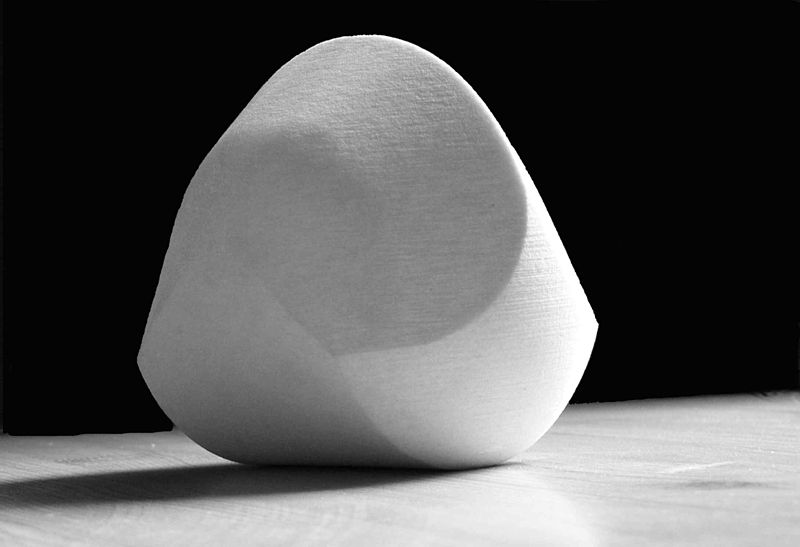
\includegraphics[scale=0.15]{Gomboc.jpg}
\caption{\label{fig:gomboc}Gömböc : un objet homogène tridimensionnel mono-monostatique. (source : Wikipedia)}
\end{figure}



\subsection{Codes}
Si vous souhaitez insérer du code dans votre rapport, invoquez les commandes : \\
 \texttt{\textbackslash lstset\{language=python\}}\\
 \texttt{\textbackslash lstinputlisting[caption=\{Titre du listing\}, label=\{lst:code\}]\{./code/code.py\}}


La première commande sélectionne le langage, pour que les mots clés de celui-ci soient correctement détectés et mis en valeur. 
La seconde commande permet d'insérer le code contenu dans le fichier code.py qui se trouve dans le sous-répertoire code.
Pour faire référence au code, il suffit de sélectionner le label du listing \ref{lst:prime},  comme pour les figures et les tableaux.

\lstset{language=python}
\lstinputlisting[caption={Titre du listing}, label={lst:prime}]{./code/primegen.py}


\subsection{Index et glossaire}

Pour insérer des entrées dans l'index, il suffit de déclarer des mots via la commande \texttt{\textbackslash index\{Fabrication d'un index\}} comme suit\footnote{Allez donc voir l'index \ref{sec:index} à la fin du document  !}. \index{Fabrication d'un index}

Pour utiliser le glossaire, il faut définir les termes dans le fichier \texttt{glossaire.tex} en utilisant la commande \texttt{\textbackslash newacronym\{label\}\{abbréviation\}\{Signification\}}. 
Puis,  \texttt{\textbackslash gls\{label\}} permet de les utiliser dans le document. 


Par exemple, les UVs 3.4 et 4.4 sont une initiation à l'\gls{IS}. 
Un concept de gestion de projet souvent mal connu est le \gls{WBS}.


\section{Références bibliographiques}

Les références bibliographiques sont des documents numériques, des livres, des articles, des images ou des vidéos qui ne sont pas présents dans le rapport. 
\LaTeX propose un mécanisme simple de citation.
Pour plus de détails, vous pouvez consulter les références suivantes \cite{maguis2010redigez,desgraupes2003latex,bitouze2010latex} qui sont présentent à la médiathèque de l'ENSTA Bretagne, ou celle-ci directement sur le web \cite{openclassroomLaTeX}.  

Pour citer des documents, il suffit d'appeler la commande \texttt{\textbackslash cite\{key\}} en choisissant la clé qui identifie le document, comme suit : \cite{lamport1985i1}. 
Cette clé de citation est celle qui référence l'ouvrage dans le fichier de bibliographie intitulé   \texttt{bibliographie.bib}.
Ce fichier d'exemple contient tous les types de documents dont vous aurez besoin : livre, article de journal, références web,  rapport\dots 
Une fois insérée et compilée, la citation devient un lien dans le fichier pdf, redirigeant ainsi directement vers le détail de l'ouvrage cité dans la bibliographie située à la fin du document.
 


\mainmatter       % La partie principale du document

%----------------------------------------------------------------------------------------
%	PART I 
%----------------------------------------------------------------------------------------
\part{Introduction au projet}
\chapter{Formulation initiale du projet}



\section{Contexte}

BeeHive Monitoring System (BMONS) est un projet qui a pour but d'aider les apiculteurs. Il s'agit de leur proposer un système de surveillance et de détection peu onéreux afin de prodiguer les meilleurs soins au meilleur moment aux ruches qui en ont besoin et d'éviter les vols.

En effet, les abeilles sont vitales à l'équilibre écologique. Einstein avait même dit: " Si l’abeille disparaît, l’humanité en a pour quatre ans à vivre ". Sans elles 84 \% des espèces végétales cultivées pour l'alimentation disparaitraient. Or les abeilles sauvages sont aujourd'hui rares et l'espèce ne survivrai pas sans l'aide des apiculteurs. Ainsi le travail de ces derniers est crucial non seulement pour assurer la production de miel mais aussi pour la sauvegarde de l'environnement. Cependant, ces dernières années, les apiculteurs ont été confrontés à de nombreux problèmes et nous sommes aujourd'hui face à une diminution du nombre d'abeilles telles que la production annuelle européenne de miel est quatre fois moindre que celle d'il y a vingt ans. 

Pour aider à la résolution de ce problème, nous voulons donc créer un système capable d'aider l'apiculteur dans son travail et de ce fait combattre la disparition des abeilles. 

\section{Expression initiale du besoin}

Après avoir discuté avec plusieurs apiculteurs, nous avons pu identifier leurs besoins et déterminer de quelle manière nous pouvons les aider. Ainsi l'objectif de ce système est tout d'abord de donner accès à l'apiculteur à des informations clés sur la ruche sans que celui-ci n'ai à se déplacer, ni à ouvrir les ruches. En effet l'ouverture de la ruche perturbe les abeilles et elle n'est pas possible en hiver à cause des températures trop basses. De plus les ruches sont souvent disposées dans des ruchers éloignés les uns des autres, ce qui complique le travail de l'apiculteur. Les informations nécessaires seraient : la température dans et en dehors de la ruche, le poids, l'humidité et les sons de la ruches. Mais le système devra aussi alerter l'apiculteur quand la sécurité de la ruche est compromise, pour permettre une action rapide destinée à sauver la colonie.

Le système BMONS est donc composé de deux parties distinctes. La première consiste en un élément embarqué dans la ruche qui consomme un minimum d'énergie et qui mesure les paramètres clés. Les données de cet élément embarqué sont transmises à un serveur via un transmetteur sans fils à un serveur qui constitue la deuxième partie du système. Il donne accès à l'apiculteur aux différentes mesures effectuées dans et autour des ruches. Il envoie également des alertes de sécurités à l'apiculteur si besoin. 
\chapter{État de l'art}

Quel est l’existant ? 

Quelles sont les solutions connues (algorithmes, matériels, logiciels, comportements, stratégies) ? 

Que pourrait-on (ré)utiliser pour le projet ? 

%----------------------------------------------------------------------------------------
%	PART II 
%----------------------------------------------------------------------------------------
\part{Dossier fonctionnel}
\chapter{Ingénierie des exigences}
\section{Approche Top-Down}
\vspace{1.5cm}
Dans cette partie nous allons analyser notre système avec une approche Top-Down. Cela signifie que nous adopterons une démarche de conception descendante. Pour cela nous avons tracé le diagramme "bête à cornes", que l'on peut voir sur la figure \ref{fig:beteacorne}. Il permet de représenter graphiquement l'expression du besoin. Comme on peut le voir sur le diagramme, le système BMONS rend service aux apiculteurs en agissant sur une ou plusieurs ruches. Il a pour but d'aider la surveillance d'un rucher et d'avertir l'apiculteur en cas de problème.


\begin{figure}[h!]
\centering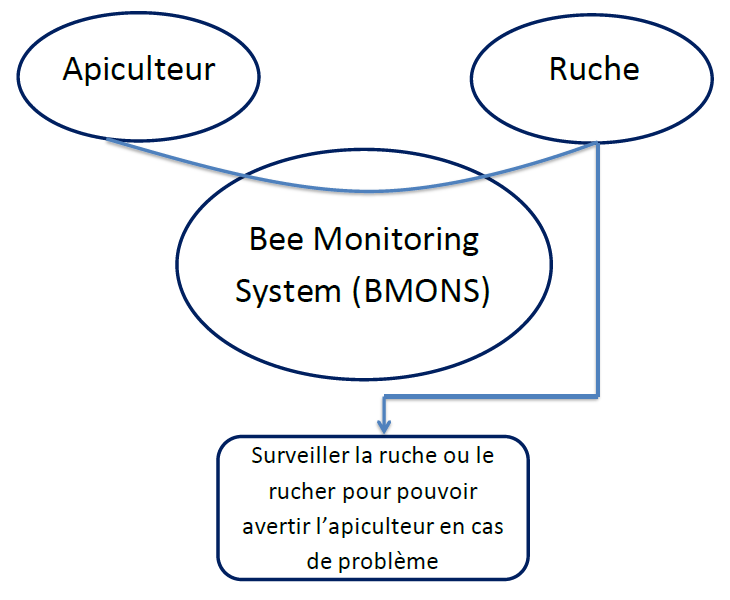
\includegraphics[scale=0.5]{BeteACornesBMONS.png}
\caption{\label{fig:beteacorne} Diagramme "bête à cornes" du système BMONS}
\end{figure}

Le diagramme pieuvre, \ref{fig:diagpieuvre1} et \ref{fig:diagpieuvre2}, nous permet ensuite de faire apparaître les fonctions principales du système. On peut aussi y retrouver les fonctions de services et de contraintes.

 
\begin{figure}[h!]
\centering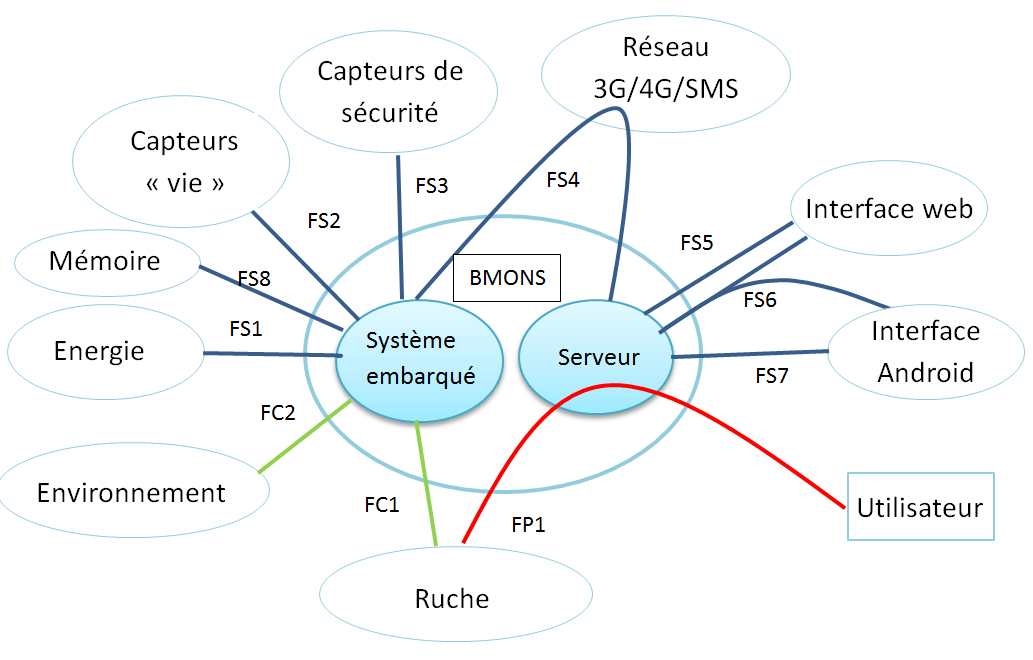
\includegraphics[scale=0.6]{pieuvre1.png}
\caption{\label{fig:diagpieuvre1} Diagramme pieuvre du système BMONS}
\end{figure}

\begin{figure}[h!]
\centering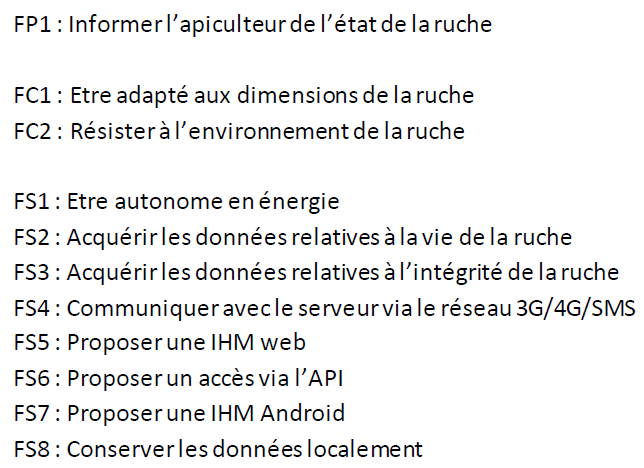
\includegraphics[trim = 1cm 0.5cm 13cm 1cm,scale=0.6]{pieuvre2.png}
\caption{\label{fig:diagpieuvre2} Légende diagramme pieuvre du système BMONS}
\end{figure}

\clearpage

\section{Approche Bottom-Up}

\vspace{1.5cm}
Nous allons maintenant adopter la démarche inverse, mais néanmoins complémentaire, de l'approche Top-Down. Il s'agit de l'approche Bottom-Up. C'est une démarche de conception ascendante qui va nous permettre d'avoir une vision plus globale du système. On peut voir sur \ref{fig:exi1} et \ref{fig:exi2} les exigences issues de cette analyse.

 
\begin{figure}[h!]
\centering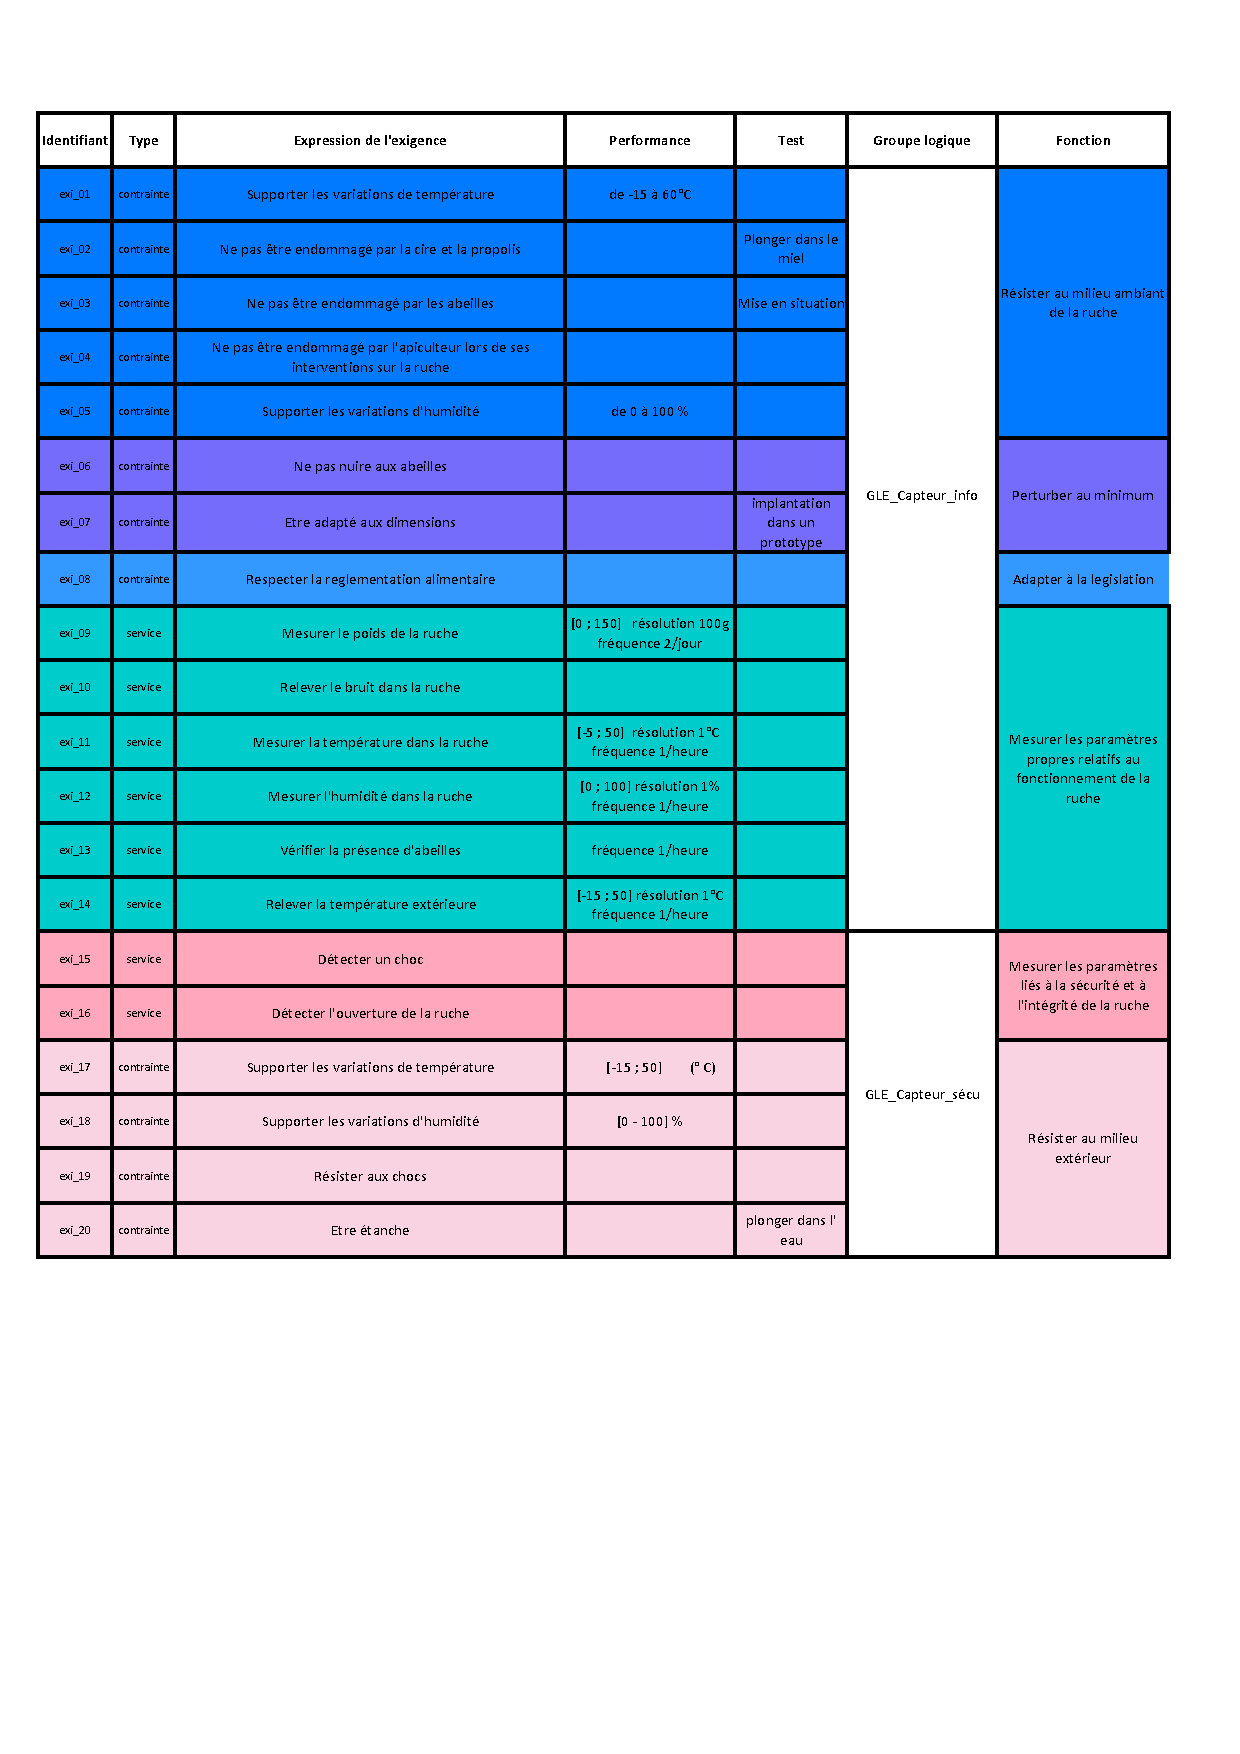
\includegraphics[trim = 1cm 8.7cm 1cm 1cm,scale=0.8]{Exigences_du_Projet_1.pdf}
\caption{\label{fig:exi1} Exigences issues de l'approche Bottom-Up (1/2)}
\end{figure}

 
\begin{figure}[h!]
\centering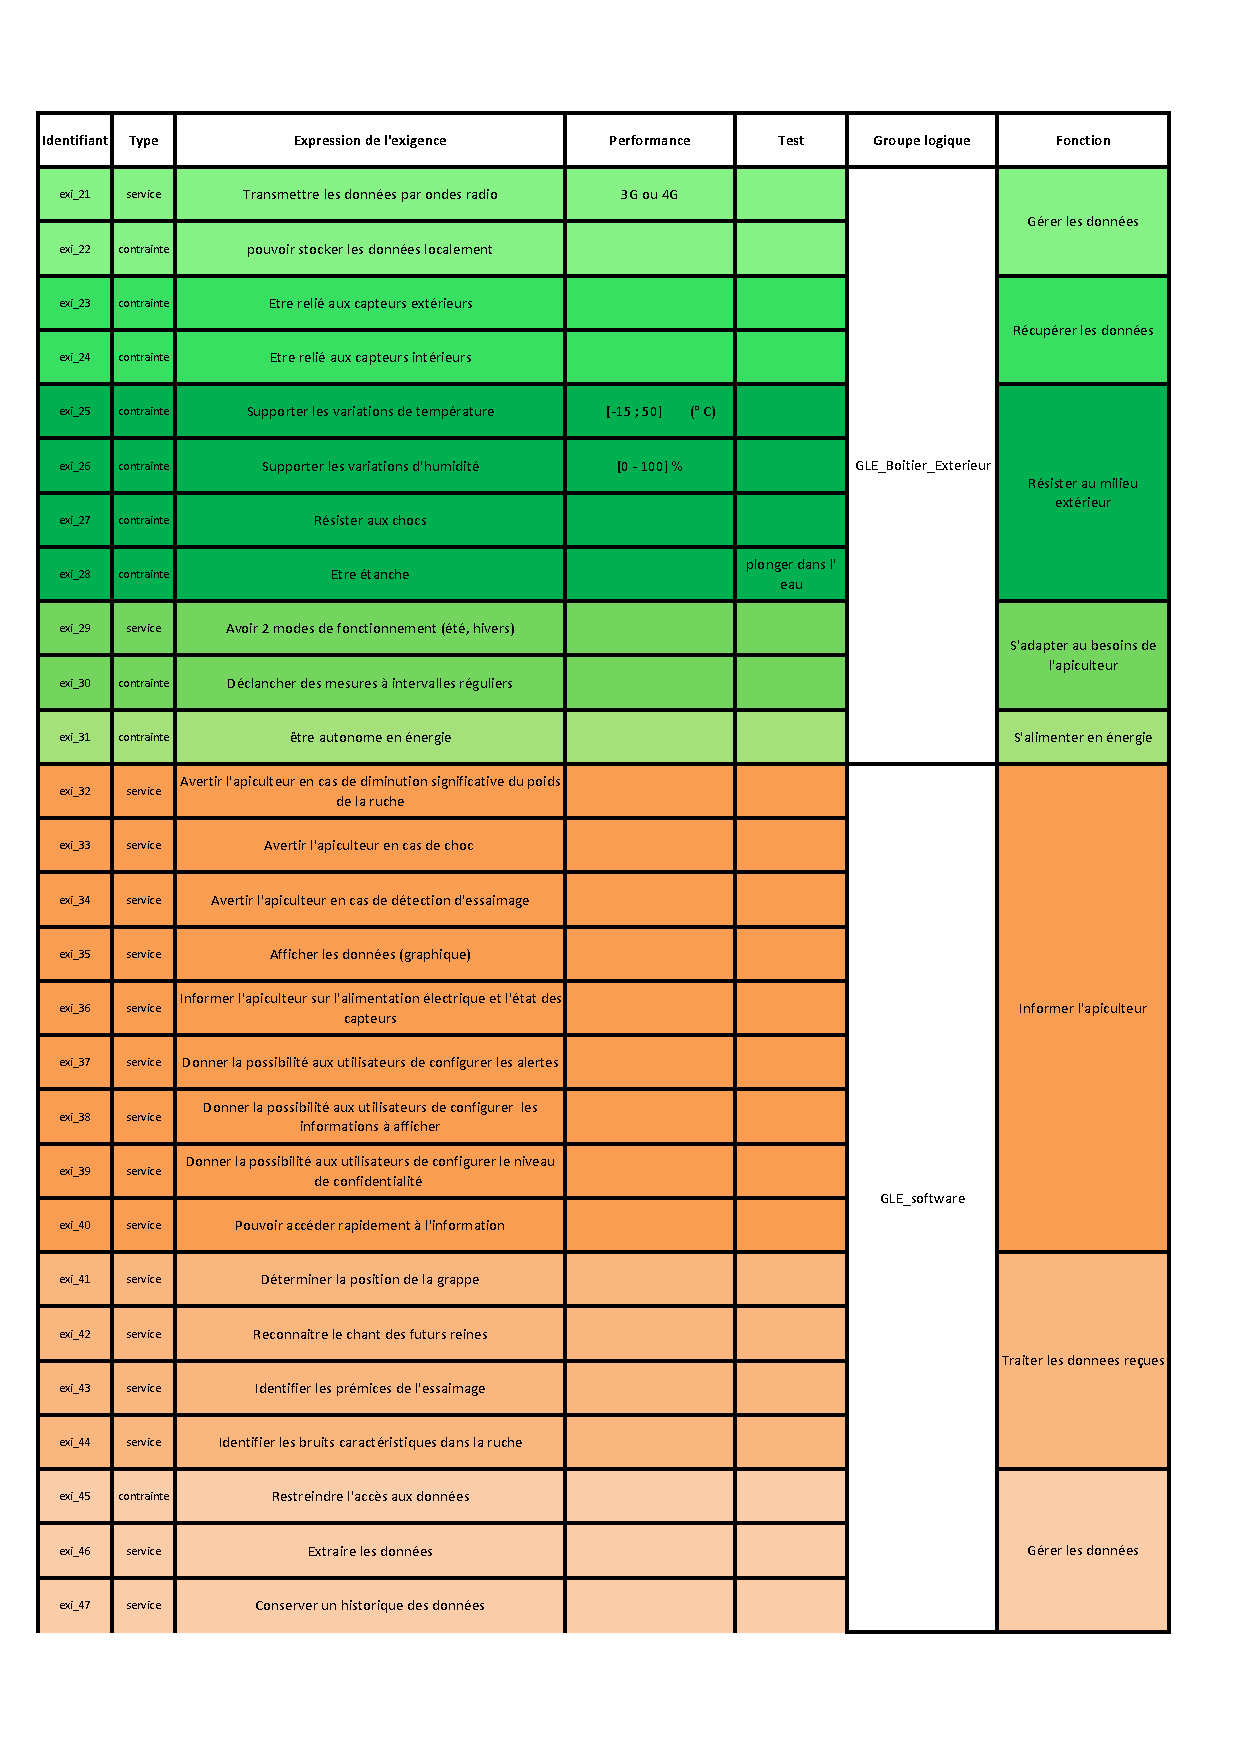
\includegraphics[trim = 1cm 2cm 1cm 1cm,scale=0.8]{Exigences_du_Projet_2.pdf}
\caption{\label{fig:exi2} Exigences issues de l'approche Bottom-Up (2/2)}
\end{figure}

\clearpage

\section{Fonctions métiers du système}
\vspace{1.5cm}

Après avoir réalisé une approche du point de vue "concepteur" du système, nous allons maintenant nous intéresser à la formulation des fonctions qu'un apiculteur souhaiterai avoir pour pouvoir suivre l'évolution de son rucher. Ces fonctions métiers ont été discutées avec notre "client", M. SINGHOFF. Elles sont présentent sur les figures \ref{fig:exi1},\ref{fig:exi2},\ref{fig:exi3} et \ref{fig:exi4}.

\begin{figure}[h!]
\centering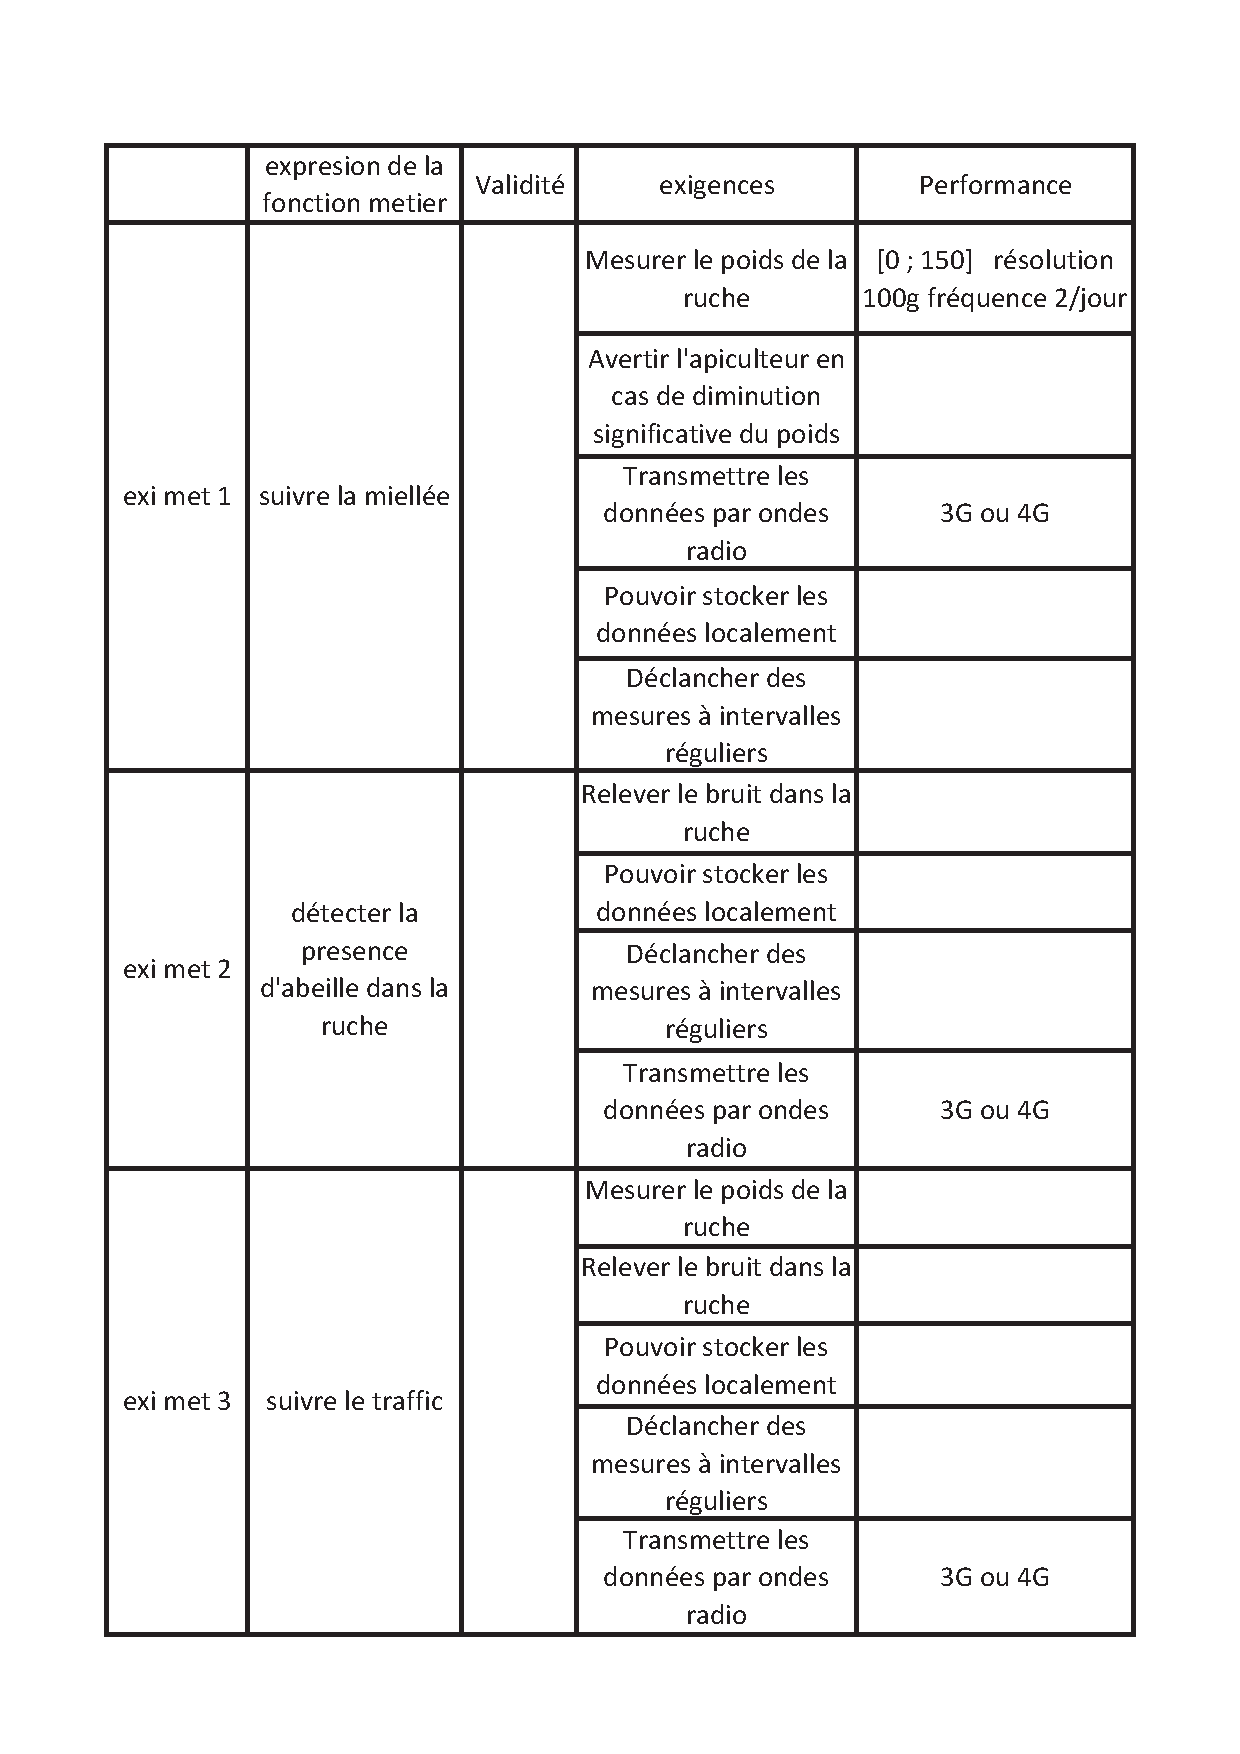
\includegraphics[trim = 1cm 2cm 1cm 1cm,scale=0.8]{Exigences1.pdf}
\caption{\label{fig:exi1} Fonctions métiers du système (1/4)}
\end{figure}

\begin{figure}[h!]
\centering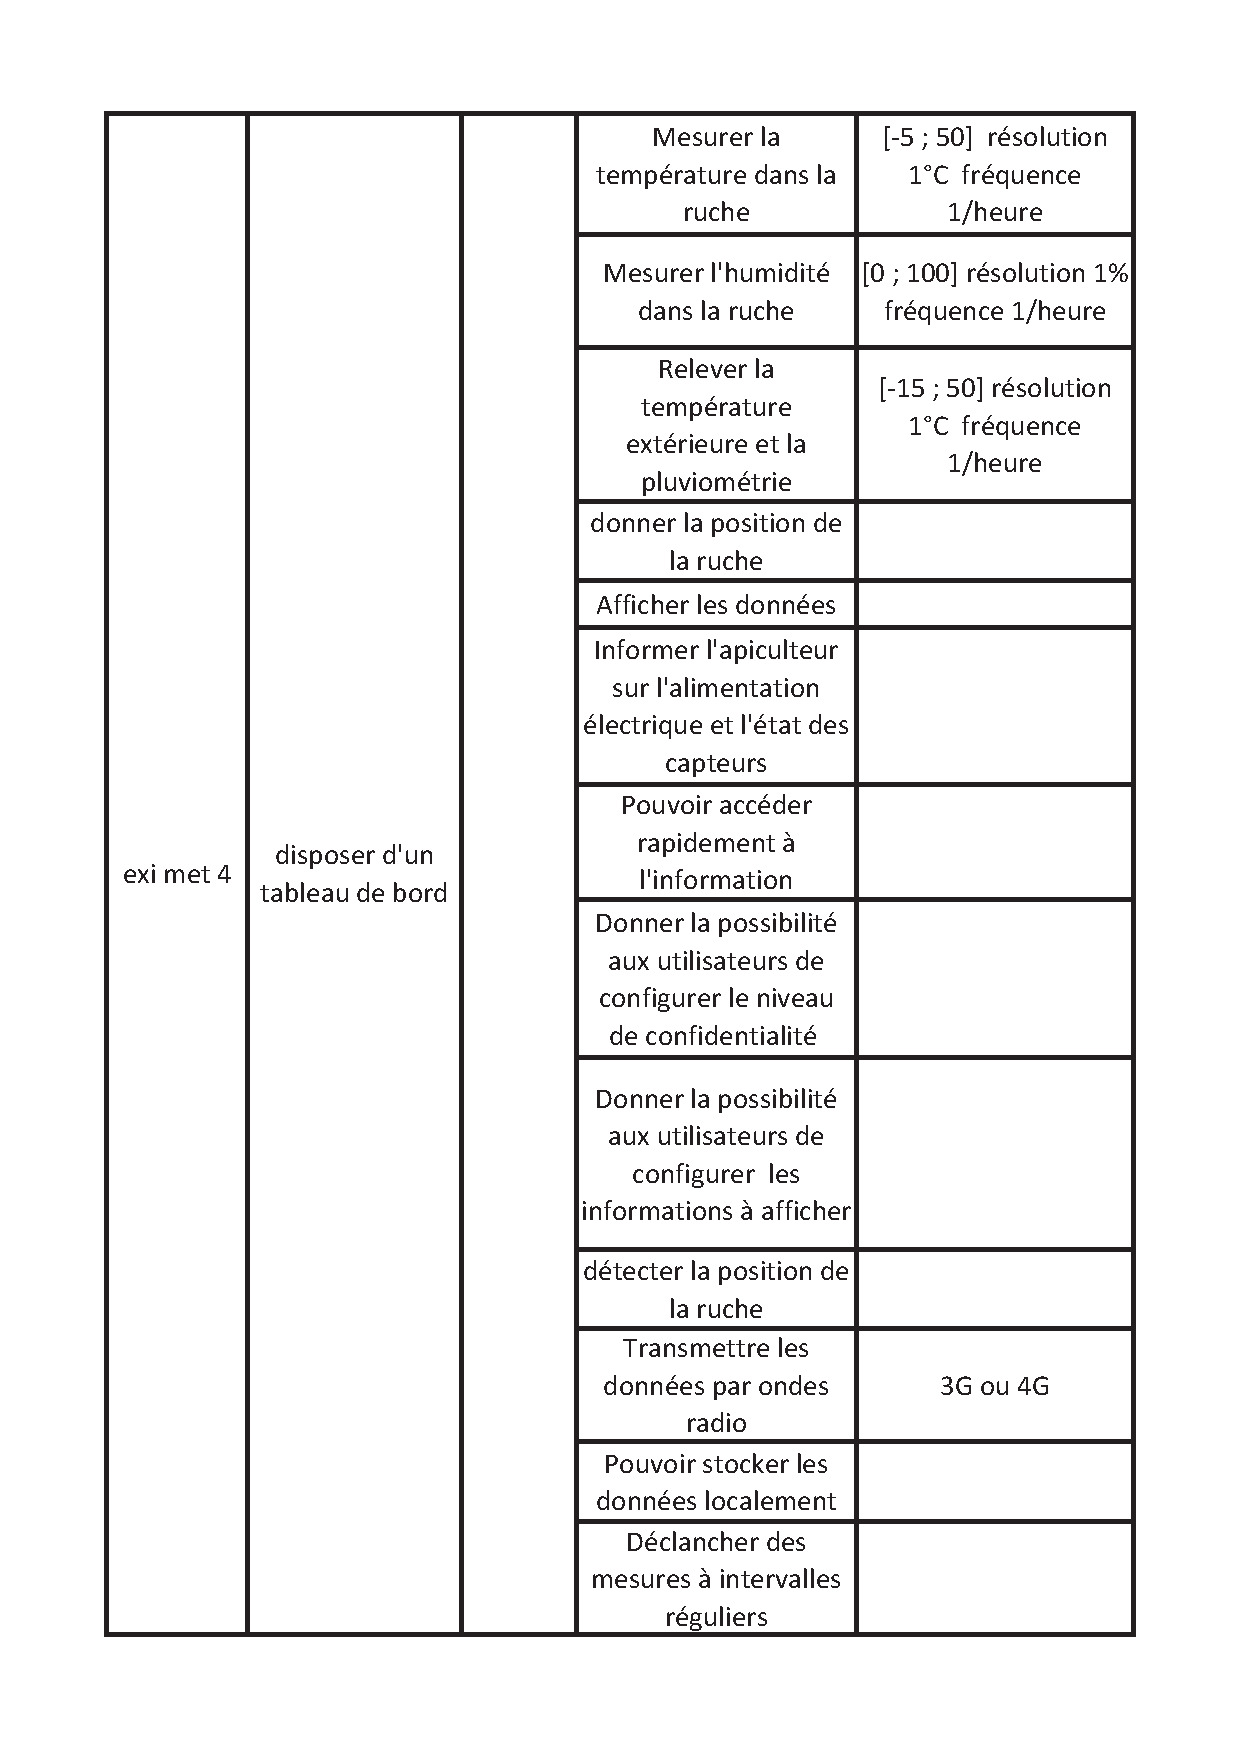
\includegraphics[trim = 1cm 2cm 1cm 1cm,scale=0.8]{Exigences2.pdf}
\caption{\label{fig:exi2} Fonctions métiers du système (2/4)}
\end{figure}

\begin{figure}[h!]
\centering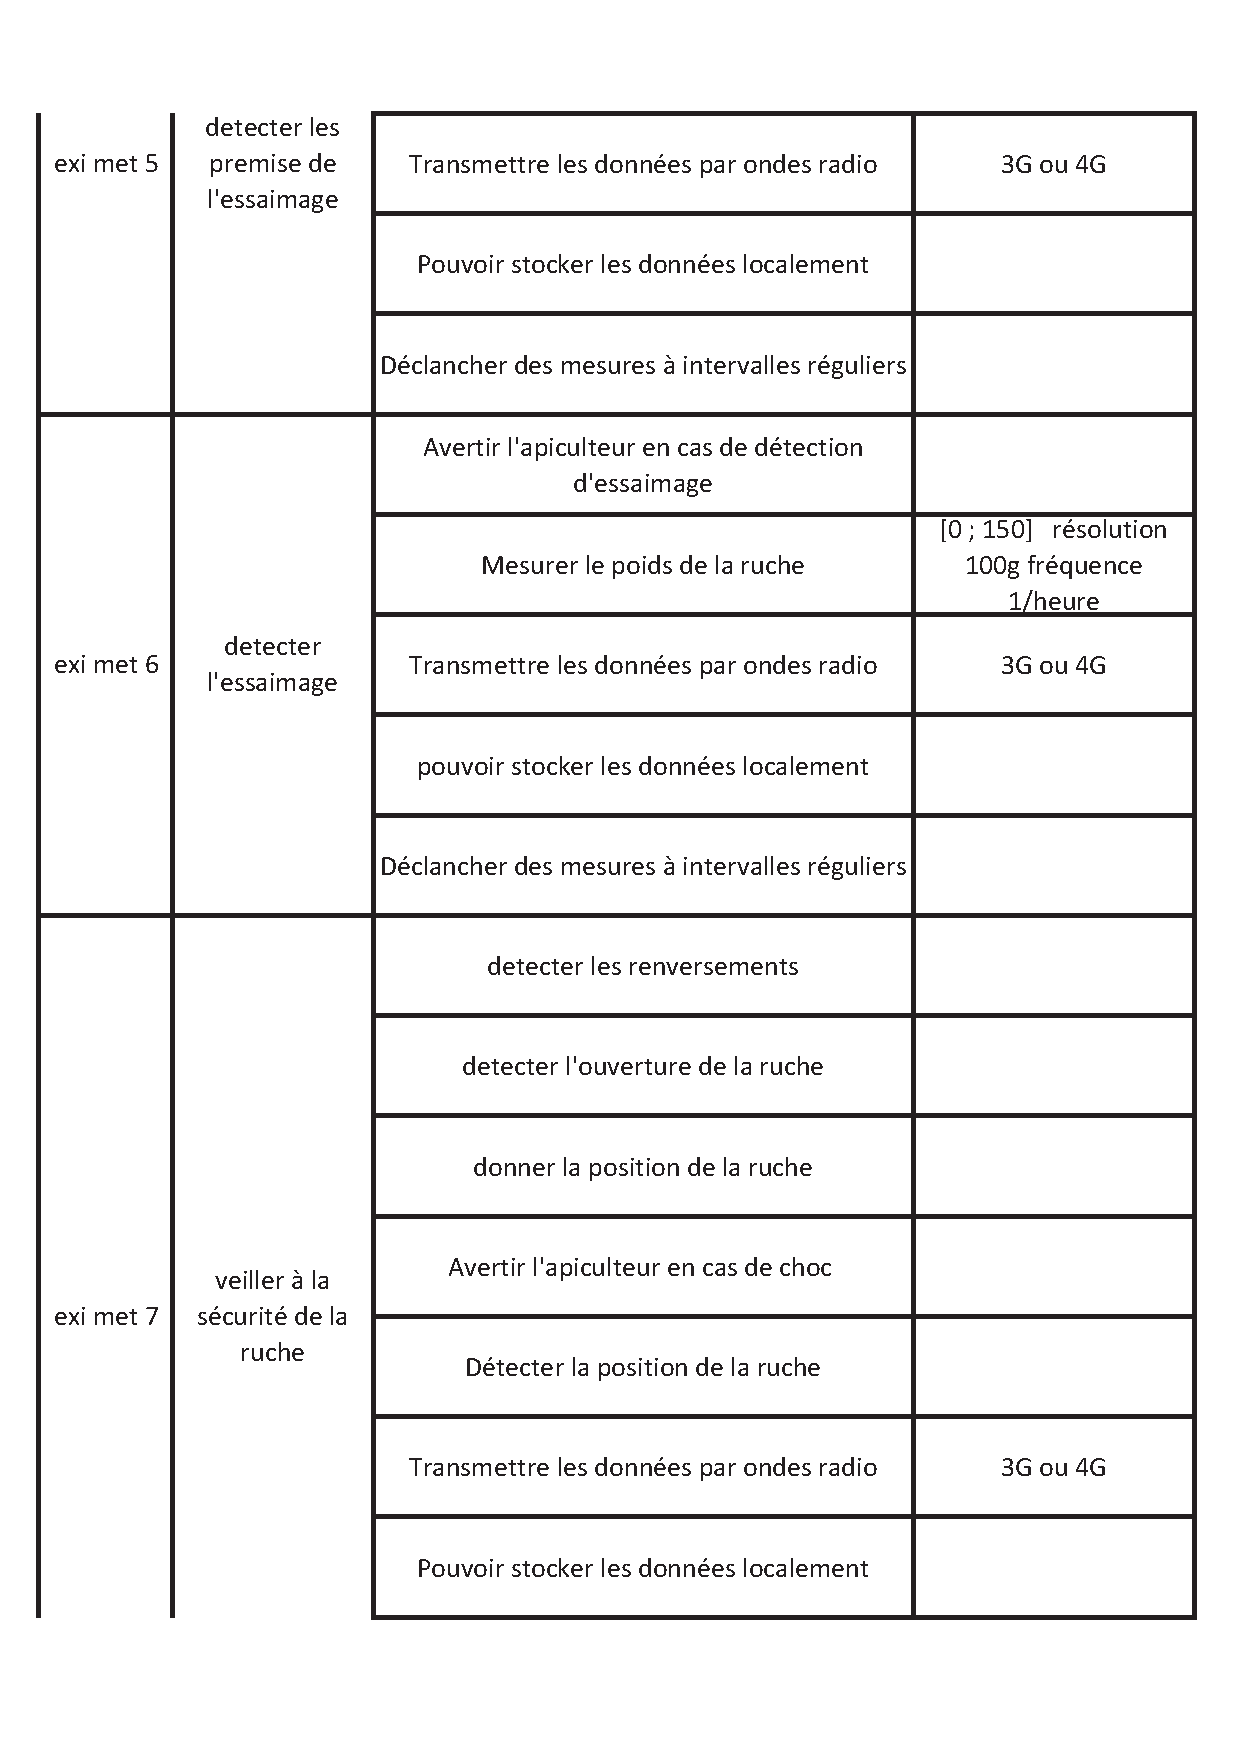
\includegraphics[trim = 1cm 2cm 1cm 1cm,scale=0.8]{Exigences3.pdf}
\caption{\label{fig:exi3} Fonctions métiers du système (3/4)}
\end{figure}

\begin{figure}[h!]
\centering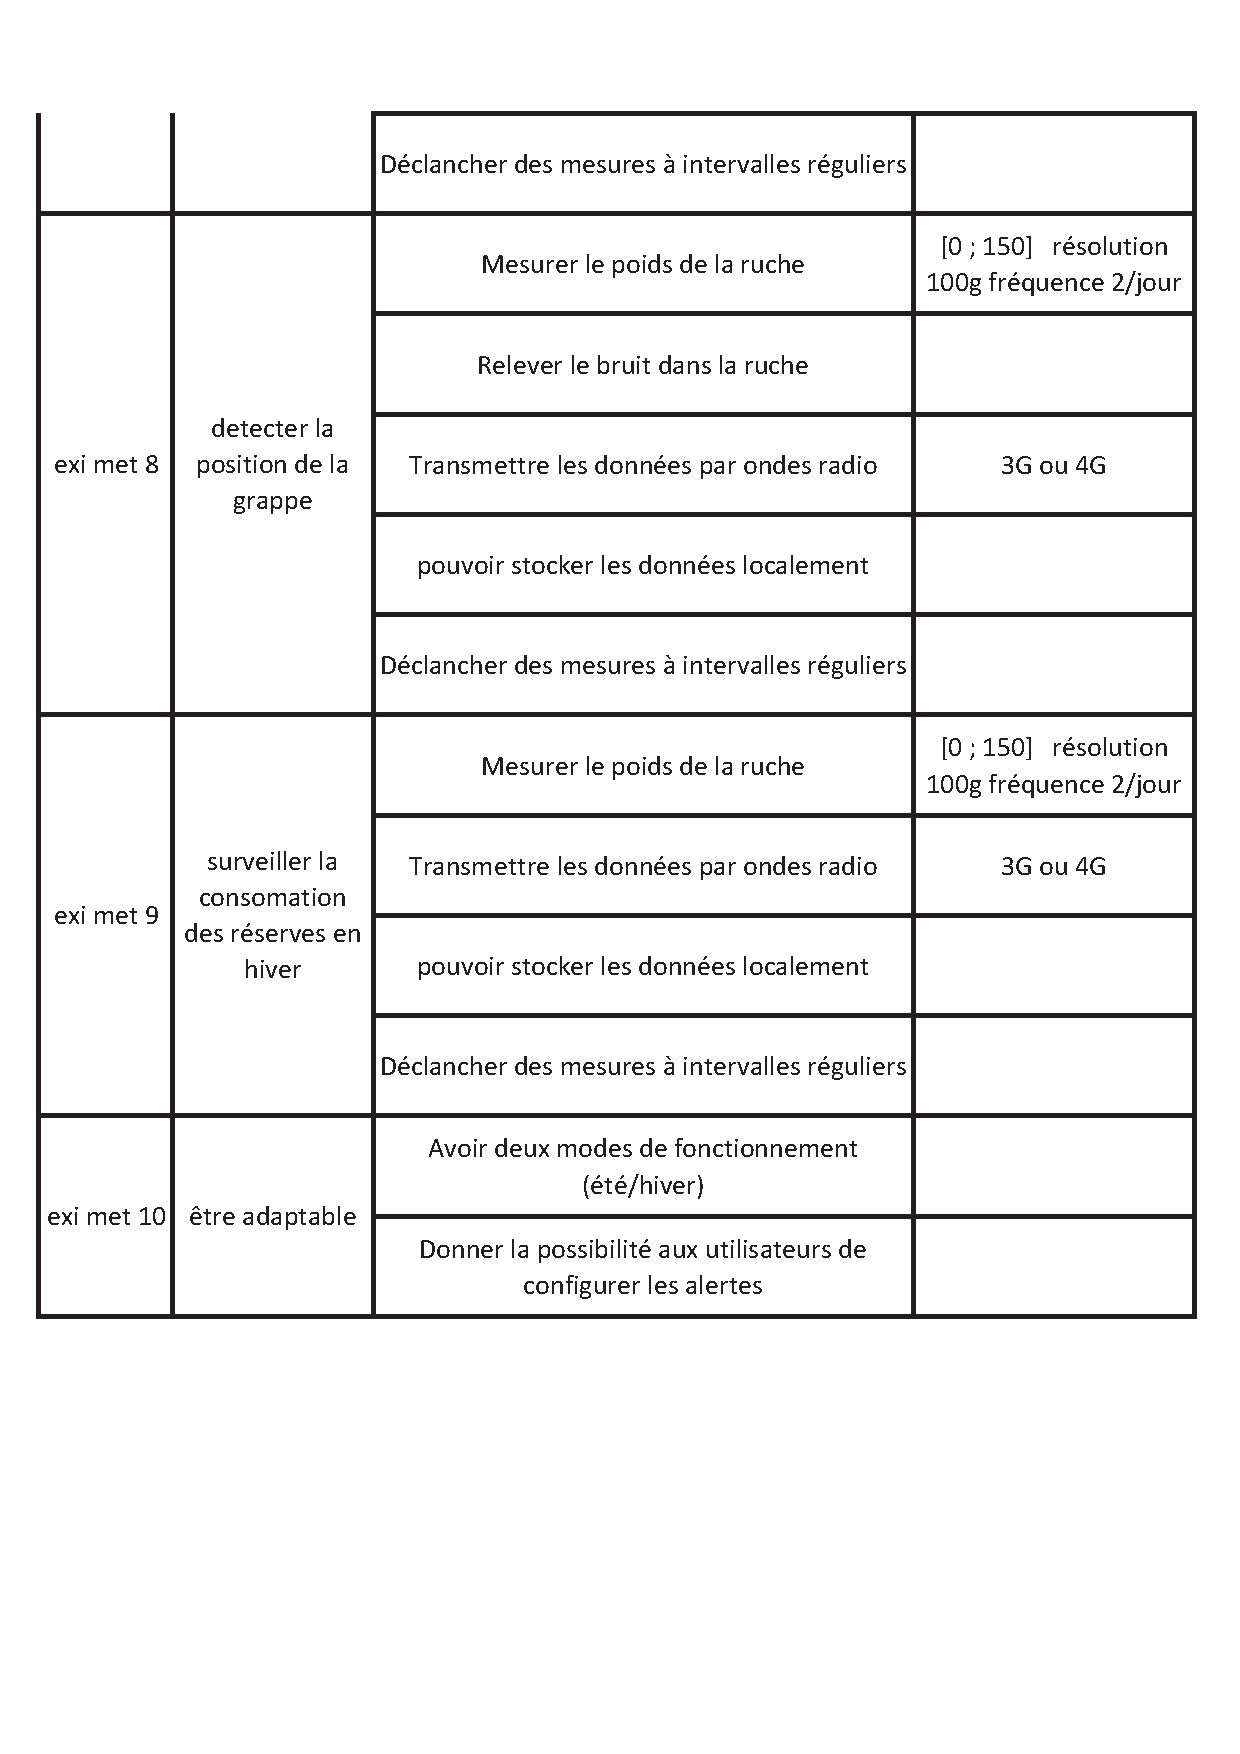
\includegraphics[trim = 1cm 2cm 1cm 1cm,scale=0.8]{Exigences4.pdf}
\caption{\label{fig:exi4} Fonctions métiers du système (4/4)}
\end{figure}

\chapter{Spécification fonctionnelle  3 axes}

\section{Raffinement FAST}
\vspace{1.5cm}
Le diagramme FAST regroupe les fonctions principales, techniques et contraintes globales définies dans lors de 
l'établissement des exigences et après leur discussion avec le client. Ainsi, certaines exigences que nous avons préalablement établit ont été acceptée mais d'autres ont écartée comme l'analyse des odeurs dans la ruche jugée finalement trop compliquée à mettre en place et difficile à exploiter. D'autres exigences ont vu le jours après les échanges avec l'apiculteur ce qui est venus enrichir et compléter notre tableau des exigences. Le raffinement des trois types de fonctions en sous fonctions et les solutions techniques 
associées a celles-ci apparaissent également. Il a évolué au cours du projet en fonction des autres documents 
d'ingénierie système et des solutions techniques retenues. 
On peut voir la version finale du FAST sur la figure \ref{fig:fast}

\begin{figure}[h!]
\centering\includegraphics[scale=0.8]{FAST_BMONS.pdf}
\caption{\label{fig:fast} Diagramme FAST du système BMONS}
\end{figure}

\clearpage

\section{Spécification des données}
\vspace{1.5cm}
La spécification des données permet de mettre à jour les différentes grandeurs 
et unités intervenant dans notre système. Grâce à cela, nous savons exactement 
quel type de donnée traiter et comment convertir les données numériques de sortie des capteurs en grandeurs physiques facilement compréhensible pour l'apiculteur. Il faudra ensuite envoyer ces données traitées au serveur qui les stockera dans une base de données. Cette étude a aussi permis d'établir les alertes qu'il va falloir prévoir afin d'avertir le propriétaire de l'état de son rucher. Ces dernières seront aussi stockées sur le serveur qui viendront compléter l'historique de la ruche. Il est possible qu'une alerte soit envoyée après avoir effectué un recoupement d'informations Par exemple, pour alerter l'apiculteur d'un essaimage en cours, il est nécessaire de détecter une agitation dans la ruche (chant de la reine) grâce au microphone et une chute importante de la masse grâce à la balance. 

Il existera deux types d'alertes: les alertes actives qui préconiserons l'apiculteur à agir directement sur la ruche (par exemple lorsque le développement de la grappe est excentrée par rapport aux cadres) et des alertes passives qui encourageront le client à se rendre sur le serveur pour consulter les derniers relevés.   

L'axe Data comportant la spécification des messages, des évènements et des alarmes est fourni en annexe.
Le diagramme des données est décris dans la figure \ref{fig:donnees} 



\begin{figure}[h!]
\centering\includegraphics[scale=0.3]{diagFluxDonnees.jpg}
\caption{\label{fig:donnees} Diagramme d'activité du flux de données}
\end{figure}

\clearpage

\section{Modèle de Données}
\vspace{1.5cm}
Le modèle de données est une façon abstraite de représenter les données du système et de modéliser les informations contenus dans une base de données. Le modèle constitue des ensembles possédant un nom et des attributs nommés. La  des relations est fait via des clés primaires (id, dans notre cas) et des clés étrangères.  

\ref{fig:UML} 



\begin{figure}[h!]
\centering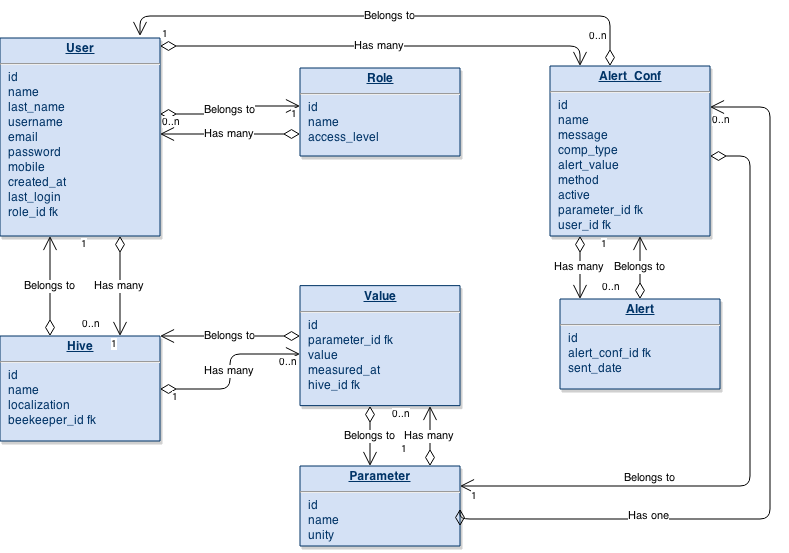
\includegraphics[scale=0.55]{UML.png}
\caption{\label{fig:UML} Modèle de données pour le système BMONS}
\end{figure}

\clearpage

\section{Spécification des comportements}
\vspace{1.5cm}
Nous allons ici décrire le fonctionnement de notre système. Il est résumé dans la figure \ref{fig:sp_comp}.

\begin{figure}[h!]
\centering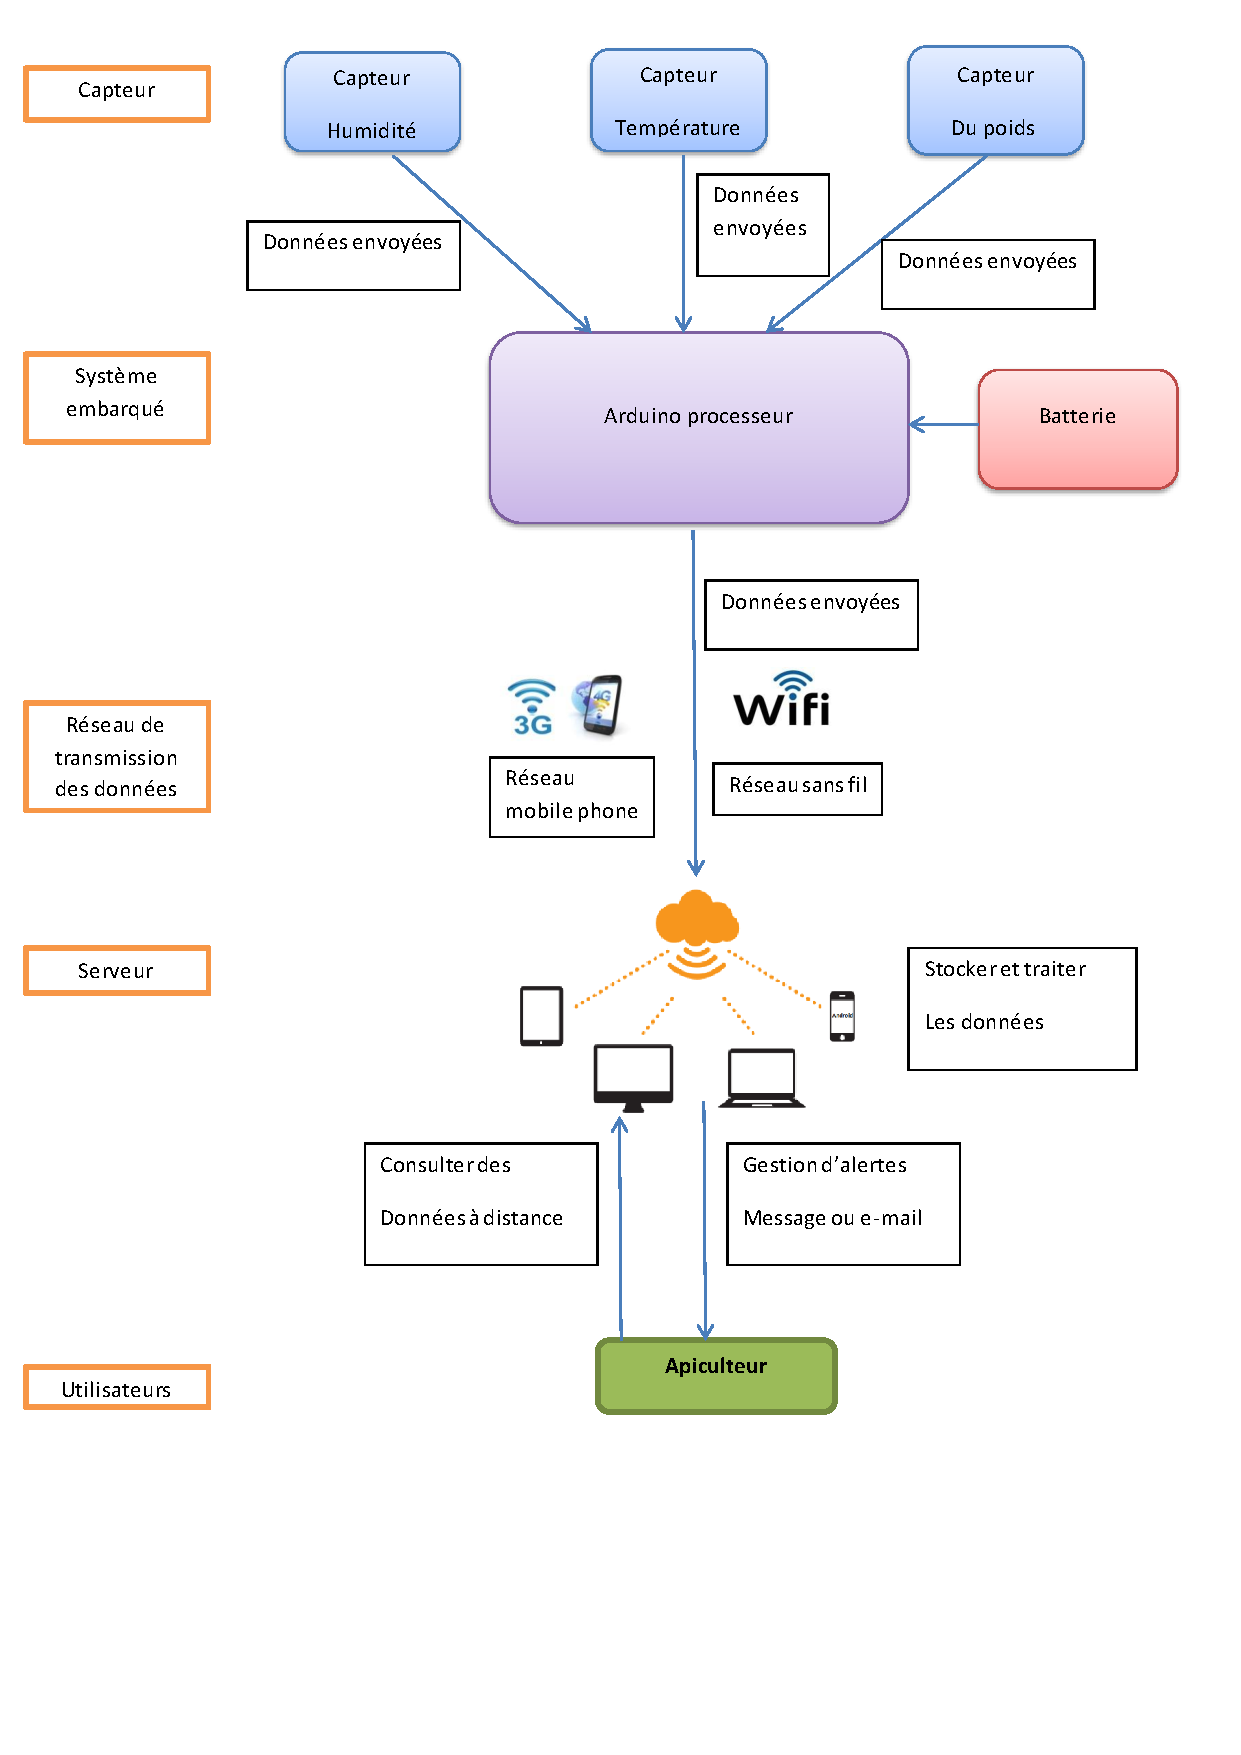
\includegraphics[scale=0.5]{specif_comp.pdf}
\caption{\label{fig:sp_comp} Diagramme de spécification des comportements}
\end{figure}

Les capteurs mesurent plusieurs paramètres internes à la ruche : l'humidité, la température et le poids de la ruche. Les données sont ensuite transmises au système embarqué. Dès que le système embarqué les reçoit, il traite les données, sélectionne celles qui sont valides et les envoi au serveur soit par le réseau sans fil (2G ou 3G), soit par le réseau téléphone si besoin. Une fois que le serveur reçoit les données, elles sont traitées et stockées dans une base de données sécurisée. Une représentation sous forme de graphiques permet une vision pratique et exploitable des informations par l'apiculteur.

Quand les mesures effectuées dépassent certain critères, par exemple, si la température est plus élevée que la température maximum pour la ruche, le serveur va générer un alerte qui sera envoyée à l'utilisateur, c'est-à-dire l'apiculteur, par SMS ou par e-mail. Par ailleurs, les apiculteurs peuvent consulter l’état de la ruche à distance afin de bien gérer la productivité de la ruche ou de limiter les situations problématiques. 

La spécification du comportement ce fait également grâce aux diagrammes de séquence. Ces diagrammes expliquent précisément comment les différent parties du système interagissent dans le but d'exécuter une action. Ils détail l'ordre des actions ainsi que leur nature et leur durée d'exécution. A ce jour 5 diagrammes de séquence ont été réalisé ils concernent l'action de récupération de la mémoire flash, l'analyse des information par le serveur, le service permettant à l'apiculteur d'avertir le serveur d'une intervention sur une ruche, la fonction permettant la configuration des alertes et l'action de connexion d'un apiculteur à son compte.
\begin{figure}[h!]
\centering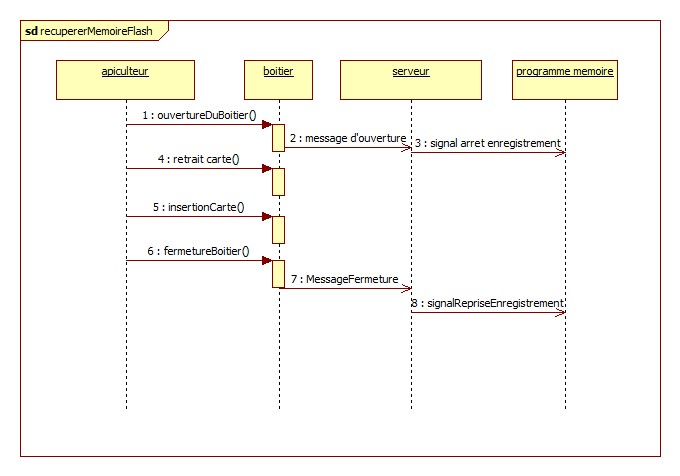
\includegraphics[scale=0.7]{recupererMemoireFlash.jpg}
\caption{\label{fig:sp_comp} Diagramme de récupération de la mémoire flash}
\end{figure}
\begin{figure}[h!]
\centering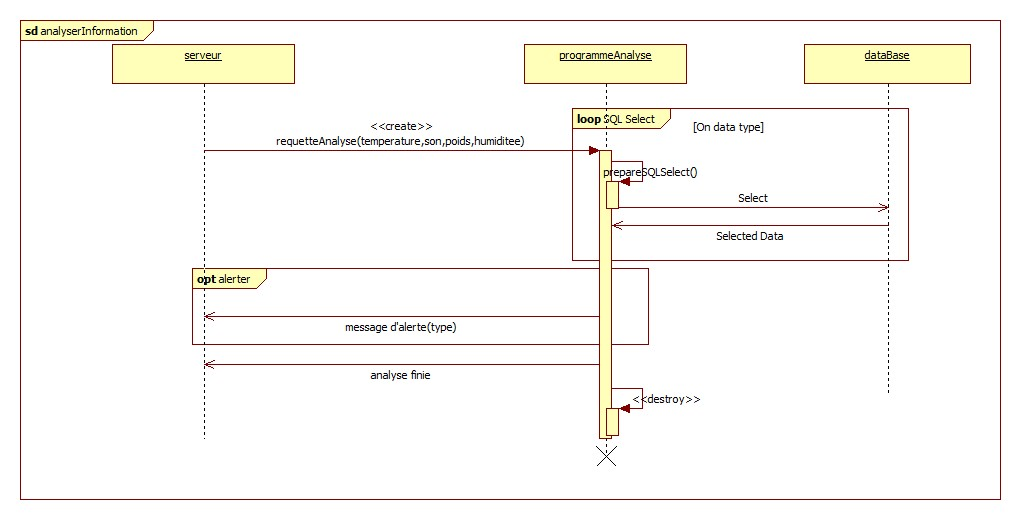
\includegraphics[scale=0.5]{analyserInformation.jpg}
\caption{\label{fig:sp_comp} Diagramme d'analyse de l'information}
\end{figure}
\begin{figure}[h!]
\centering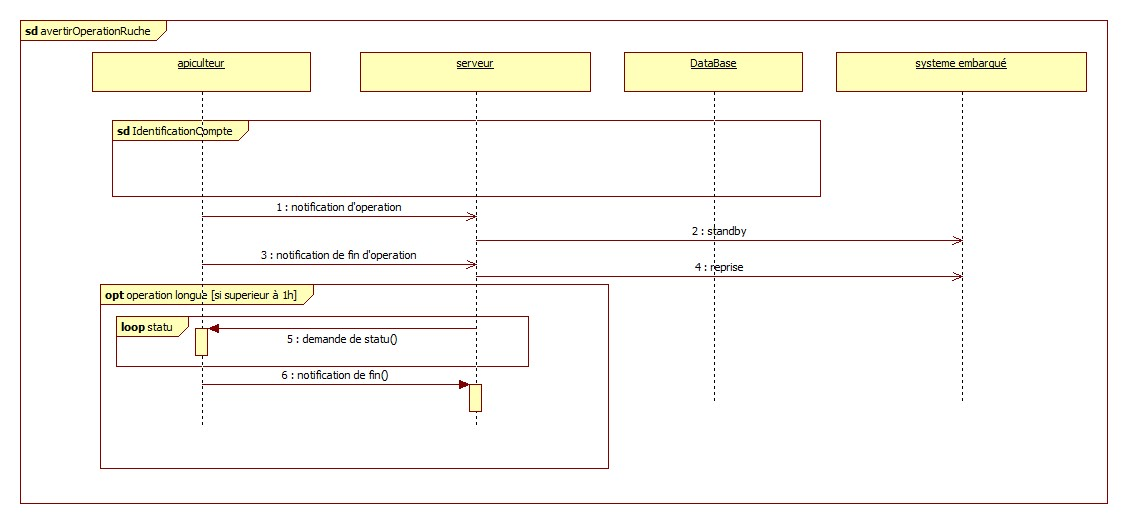
\includegraphics[scale=0.5]{avertirOperationRuche.jpg}
\caption{\label{fig:sp_comp} Diagramme d'avertissement d'opération sur la ruche}
\end{figure}
\begin{figure}[h!]
\centering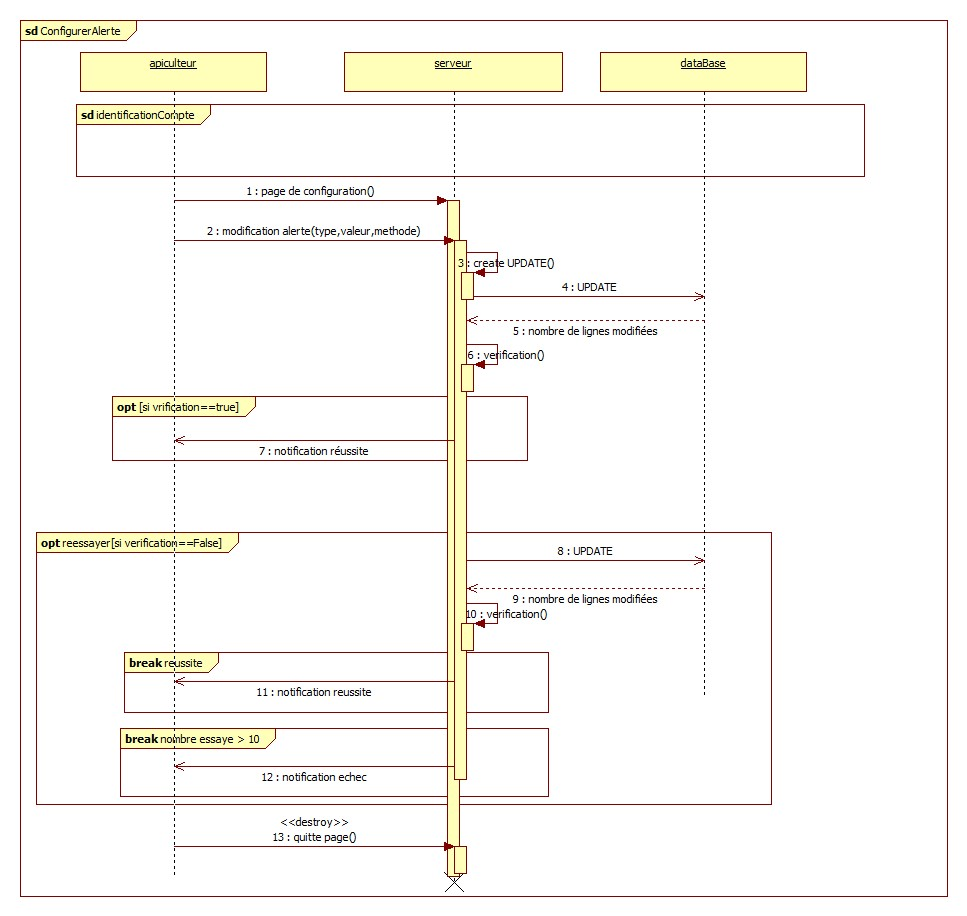
\includegraphics[scale=0.5]{configurerAlerte.jpg}
\caption{\label{fig:sp_comp} Diagramme de configuration des alertes}
\end{figure}
\begin{figure}[h!]
\centering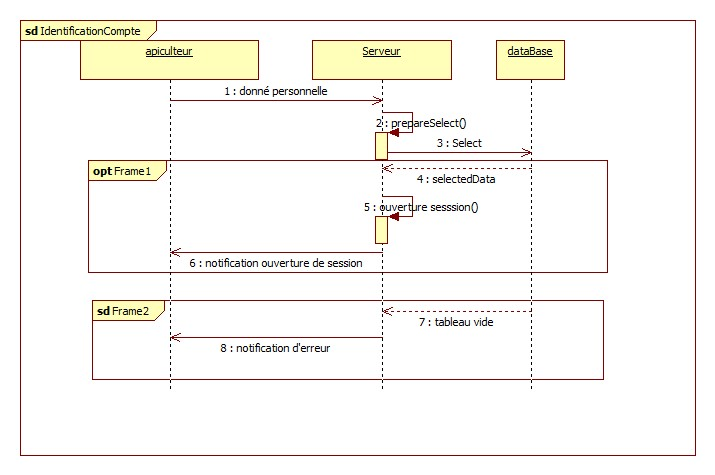
\includegraphics[scale=0.7]{IdentificationCompte.jpg}
\caption{\label{fig:sp_comp} Diagramme d'identification compte}
\end{figure}
\pagebreak

\chapter{Architecture fonctionnelle}

L'étude de la spécification fonctionnelle trois axes a permis d'établir l'architecture fonctionnelle du système qui est représentée sur la figure \ref{fig:anaFonc}.
Ce schéma résume les interactions entre chaque partie: Bee Monitor qui regroupe l'ensemble des capteurs, la carte Arduino ainsi que la carte SSD pour l'enregistrement local des données, le module de transmission et le système d'alimentation rendant notre projet autonome en énergie et le serveur. Chaque acteur interagissant avec le système y sont également représentés: Les abeilles/ruche, l'apiculteur et l'environnement.   
  

\begin{figure}[h]
\centering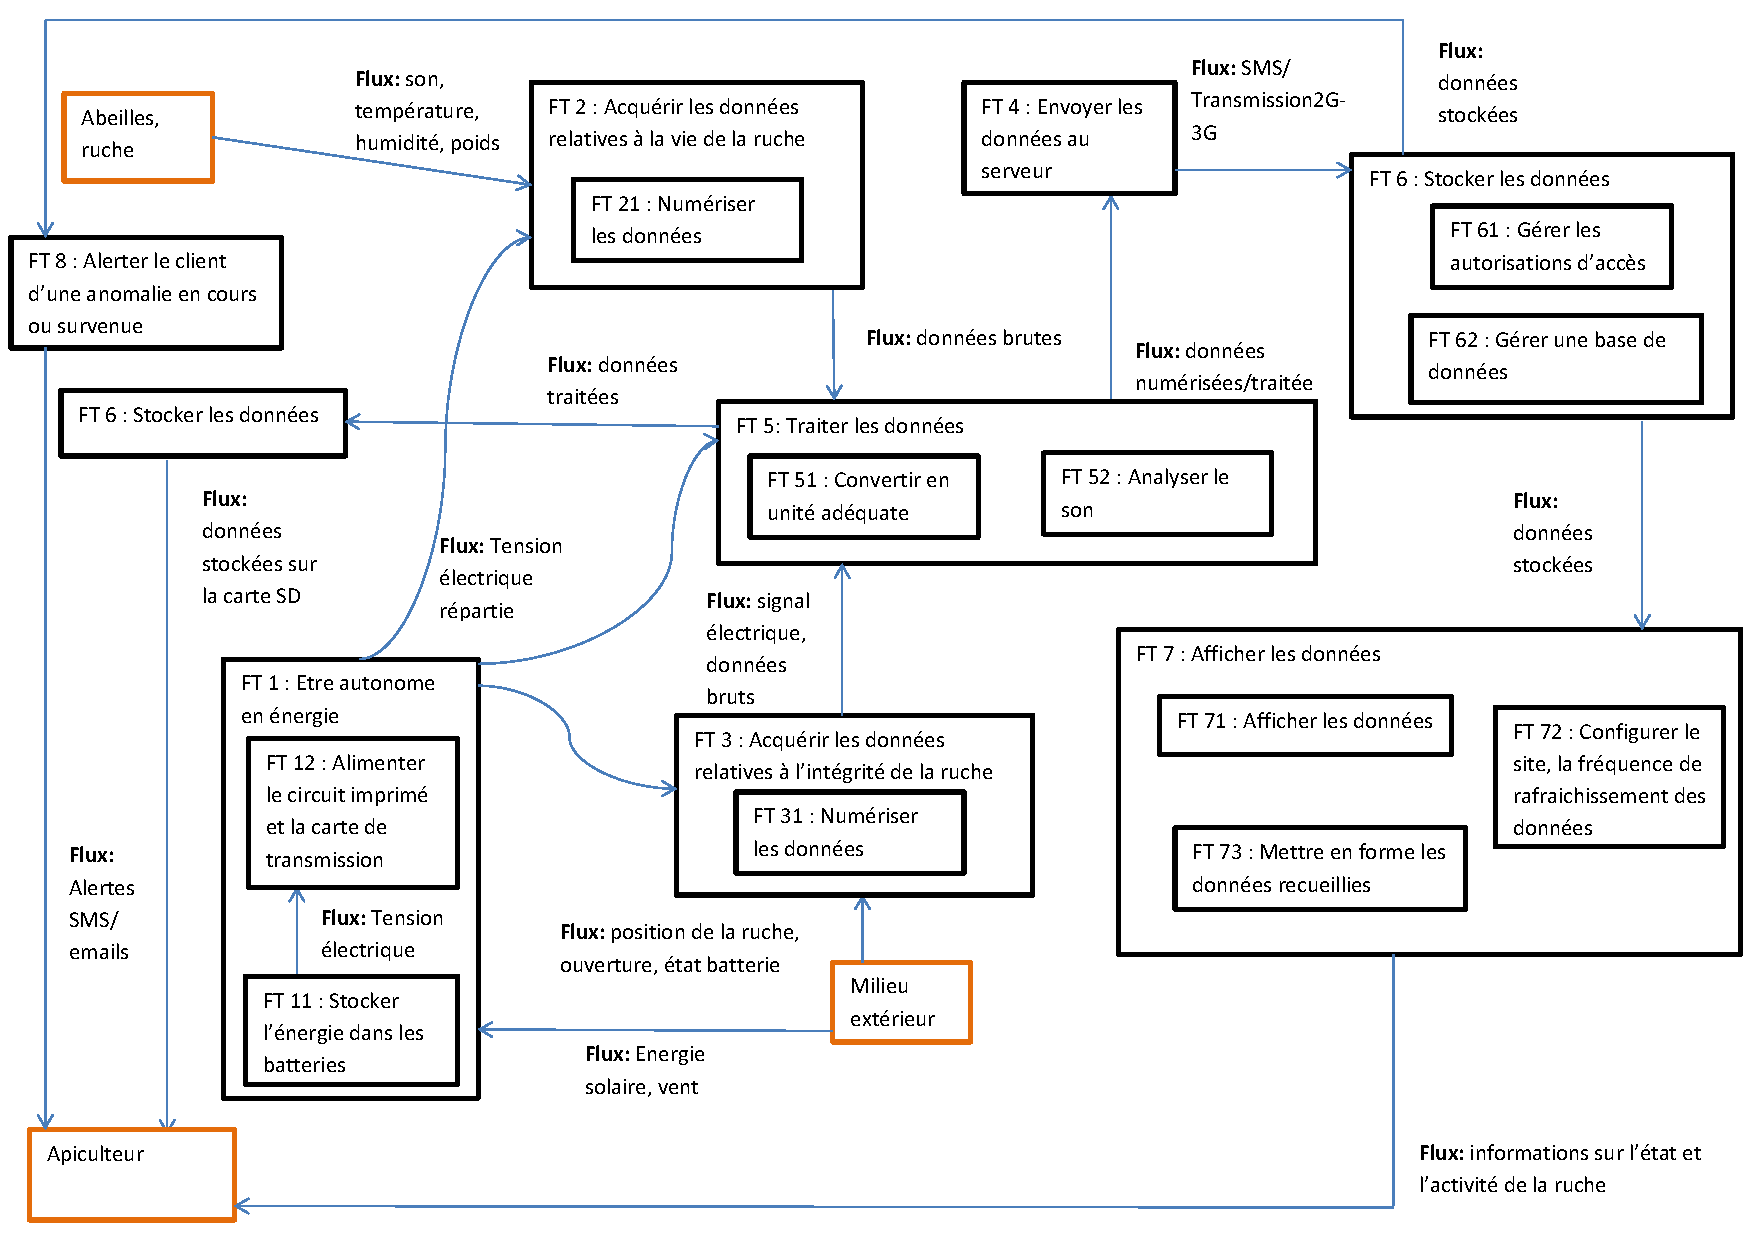
\includegraphics[scale=0.5]{analyseFonctionelle1.pdf}
\caption{\label{fig:anaFonc} Architecture fonctionnelle}
\end{figure}    



%----------------------------------------------------------------------------------------
%	PART III 
%----------------------------------------------------------------------------------------
%\part{Implémentation}
%
\chapter{Architecture physique}

\section{Architecture physique}

%\chapter{Interfaces}
%%\chapter{Structure de découpage du projet}
\section{Structure de découpage du projet}

Structure de découpage du projet, ou Work Breakdown Structure (WBS) en anglais, est un diagramme hiérarchique, axée sur les tâches et activités que l’équipe de projet doit exécuter pour atteindre les objectifs du projet.

Dans cette partie nous allons analyser nos tâches. Elles sont divisés en deux parties: Serveur et Arduino. La partie serveur comprend tout qu'est lié au développement du site et les scripts qui contrôlent les logiciels, les backups et l'obtention de données. La partie arduino comprend tous les capteurs et modules, l'énergie et les scripts de contrôle des capteurs et manipulation des données.  


\begin{figure}[h!]
\centering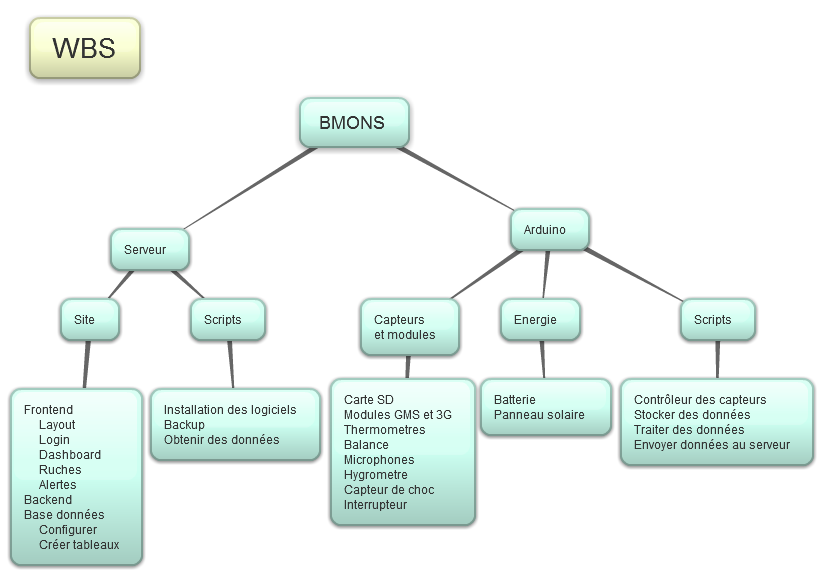
\includegraphics[scale=0.55]{WBS.png}
\caption{\label{fig:SDP} Structure de découpage du projet du système BMONS}
\end{figure}

\clearpage 
%\chapter{Tests}

Après avoir pris en main nos capteurs, nous avons prévu de tester leur validité en préparant une série de tests pour chacun d'entre eux. Cela nous permettra notamment de vérifier leur précision et les conséquences d'un dépôt de miel ou de propolis à leur surface. Ainsi, les résultats de ses test pourra affecter leur position dans la ruche. 


\section{Capteur de température}

\noindent \underline{Matériel}:  
3 capteurs de température, de la cire d'abeilles et 1 support\newline  

\noindent \underline{Préparation:} \newline 
Fixer les capteurs de température sur le support espacés de manière régulière. Sur le capteur de gauche appliquer 0.5 cm de cire et sur le capteur de droite appliquer 1 cm de cire. Le capteur central sera le témoin \newline

\noindent \underline{Test 1:} \newline 
Mettre le support au frigo et surveiller l'évolution de la température\newline   
Relever le temps nécessaire pour arriver à la même température que le témoin pour les 2 capteurs tests  

\noindent \underline{Test 2:}  \newline 
Directement après le test 1 enlever le support du frigo et surveiller l'évolution de la température\newline   
Relever le temps nécessaire pour arriver à la même température que le témoin pour les 2 capteurs tests

\noindent \underline{Test 3:}  \newline 
Mettre le support dans un "four" à 30 degrés et surveiller l'évolution de la température\newline   
Relever le temps nécessaire pour arriver à la même température que le témoin pour les 2 capteurs tests  
  
\noindent \underline{Test 4:}  \newline 
Directement après le test 3 enlever le support du "four" et surveiller l'évolution de la température\newline   
Relever le temps nécessaire pour arriver à la même température que le témoin pour les 2 capteurs tests

\newpage

\section{Capteur d'humidité} 

\noindent \underline{Matériel}: 
1 capteur d'humidité des sachets déshydratants\newline  
2 boites/sachets hermétiques cotons et eau \newline 

\noindent \underline{Préparation:} \newline  
Commencer et finir le cycle avec un capteur propre\newline  

\noindent \underline{Etape 0:}  

\noindent Relever le niveaux d'humidité d'origine  

\noindent \underline{Etape 1:} \newline  
Mettre le support dans réceptacle à 100\% d'humidité\newline  
Surveiller l'évolution\newline  
Relever les courbes

\noindent \underline{Etape 2:} 

\noindent Mettre le support dans un réceptacle à 0\% d'humidité 

\noindent \underline{Etape 3:}  \newline
Répéter les  étapes 1 et 2 cinq fois avec différentes épaisseurs


%----------------------------------------------------------------------------------------
%	PART IV 
%----------------------------------------------------------------------------------------
%\part{Intégration et validation}
%\chapter{Intégration}

%\chapter{Validation}

%----------------------------------------------------------------------------------------
%	PART V 
%----------------------------------------------------------------------------------------
\part{Organisation}
\chapter{Méthodes de travail}

% Méthodes de travail
% Organisation temporelle, spatiale, humaine 
% interactions des membres de l’équipe projet
% interactions avec les encadrants
% interactions avec les tiers

Tout au long du projet notre méthode de travail a changée. Au fur et à mesure que les séances s'enchainaient, et en prenant en compte les conseils qui nous ont été donnés (notamment à propos du carnet de bord et des objectifs à court terme) notre méthode de travail a tendu vers la suivante : \\ \\
De manière générale, toute l'équipe du projet BMONS travaille dans la même salle pour faciliter la communication entre les membres du groupe. Une séance de travail commence par l'ouverture personnelle des mails de chacun, puis le groupe se réunit pour définir les objectifs de la matinée, ensuite chacun choisit la partie il va avancer. Le travail se fait en général seul ou en binôme et des points d'avancement sont faits à l'oral tout au long de la séance. Parfois des tâches comme la prise en main d'un logiciel ou la compréhension d'un diagramme sont faites en dehors des séances, mais la majeure partie du travail s'effectue lors du temps alloué au projet. \\ \\
Les réunions avec les encadrants et les intervenants extérieurs se déroulent dans des salles de l'ENSTA Bretagne équipées d'un vidéo projecteur et en présence de la totalité de l'équipe BMONS. Ces séances sont organisées à l'avance, les points sur lesquels des précisions sont nécessaires sont mis en avant avant la séance et des questions précises sont préparées. Cela permet de guider la réunion et de ne pas perdre de temps sur des points déjà vus. Chacun a son rôle lors de ces réunions, la prise de notes, le dialogue avec l'intervenant et la rédaction du compte rendu sont ainsi facilités.


 

\chapter{Outils pour les échanges}

% Quels sont les outils qui nous permettent de travailler ensemble ?

Les outils qui nous ont permis de travailler ensemble et de partager nos fichiers ont également changés au cours du temps. 
Avant les premiers ateliers techniques, particulièrement celui sur github, nous partagions nos résultats sur le oneDrive d'office 365. \\

\chapter{Répartition des tâches dans le temps}


% WBS et diagramme de Gantt


%----------------------------------------------------------------------------------------
%	PART VI 
%----------------------------------------------------------------------------------------
\part{Journal du projet}


\chapter{Choix et justifications}

\section{Choix des capteurs}
\vspace{1.5cm}
Après avoir réalisé l'état de l'art pour notre système de surveillance d'une ruche, nous nous sommes ensuite intéressés aux capteurs que nous allons employer.\\

\textbf{Capteur de température}\\

Nous avons choisis un capteur de température identique pour recueillir la température interne et externe de la ruche.
Il s'agit d'une thermistance NTC boitier Goutte Radial 1000 ohms sortie fil de cuivre émaillé 1 pc(s). Ce dernier possède une gamme de mesure comprise entre -40 C et 100 C ce qui correspond bien aux exigences discutées avec le client (Voir tableau des exigences). Le capteur placé à l'extérieur nous renseignera sur les conditions météorologique et expliquer une éventuelle diminution de la production de miel par exemple. Celui placé à l'intérieur nous donnera une idée de l'isolation de la ruche en hiver et de sa ventilation en été.\\  

\textbf{Capteur d'humidité}\\

On a choisit d'inclure ce capteur dans notre système compte tenu des résultats de l'état de l'art. Néanmoins, après discussion avec le client, cette option n'est pas primordiale pour un apiculteur mais elle sera tout de même rajoutée au tableau de bord du serveur.\\

\textbf{Capteur de pression}\\

Les capteurs de pression vont nous permettre de récupérer le poids de ruche et surtout celui des hausses pour avertir l'apiculteur de la quantité de miel produite. Pour se faire, le projet Bzzz développé par le Fablab de Lannion a prévu d'utiliser deux sachets de "Pompote" remplis d'eau sucrée pour éviter les variations de pression atmosphérique, le gel et l'évaporation. Cependant, après avoir pris conscience de l'importance de la localisation de la grappe, nous avons pensé installer deux capteurs de pression par cadre (au niveau de chaque extrémité) soit 20 au total mais cette solution s'est avérée être difficile à mettre en place à cause de la surface sur laquelle repose les cadres (simple lamelle en métal). Après discussion avec le client, nous avons finalement opté pour la confection d'un cadre en bois aux même dimensions de la ruche dans lequel se trouverons les capteurs de pression. L'utilisateur décidera de l'endroit où le placer en fonction des données qu'il veut récupérer. 
On pourra aussi utiliser ce capteur pour détecter l'ouverture du couvercle à cause du vent.\\

\textbf{Tilt sensor}\\

Ce capteur permet de savoir si la ruche a reçu un choc ou si elle a été déplacé. Il renvoi une information binaire qui pourra être couplée avec les données de la carte GPS et ainsi avertir l'apiculteur en cas de détérioration, renversement ou vol de la ruche. Ce dernier évènement étant de plus en plus fréquent.
Nous avons choisit le TikerKit Tilt Sensor \ref{fig:tiltSensor}.\\

\begin{figure}[h]
\centering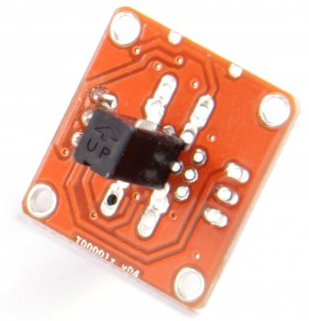
\includegraphics[scale=0.5]{tiltSensor.png}
\caption{\label{fig:tiltSensor} TikerKit Tilt Sensor}
\end{figure} 
     

\textbf{Microphone}\\

L'utilisation d'un microphone s'est imposée comme une nécessité dans la surveillance d'une ruche car il permet de recueillir des données pouvant avertir l'apiculteur sur plusieurs types d'évènements. En effet, grâce à ce dernier, on pourra détecter la présence d'abeilles dans la ruche notamment en hiver et éventuellement recueillir la source du bourdonnement et ainsi localiser la grappe approximativement. On pourra aussi détecter les prémisses d'un essaimage en percevant le champs d'une raine caractéristique de ce type d'évènement. Cette information pourra ensuite être couplée avec les données des capteurs de pression et confirmer l'essaimage en cours si le poids chute brutalement. 
Nous avons choisit le Capsule micro pour CI 2 V/DC sensibilité 44 dB (à 3 dB près) sur la plage 100 - 10000 Hz. 

\section{Choix de la carte Arduino}
\vspace{1.5cm}

Compte tenu du fait que nous avions besoin d'un nombre d'entrées assez élevé (au moins 20) ainsi que d'un temps ADC supérieur ou égal à 5kHz. Nous avons alors sélectionné quatre cartes, que nous avons ensuite comparées. Ces résultats sont regroupés dans la Figure\ref{fig:choixardui}.

\begin{figure}[h]
\centering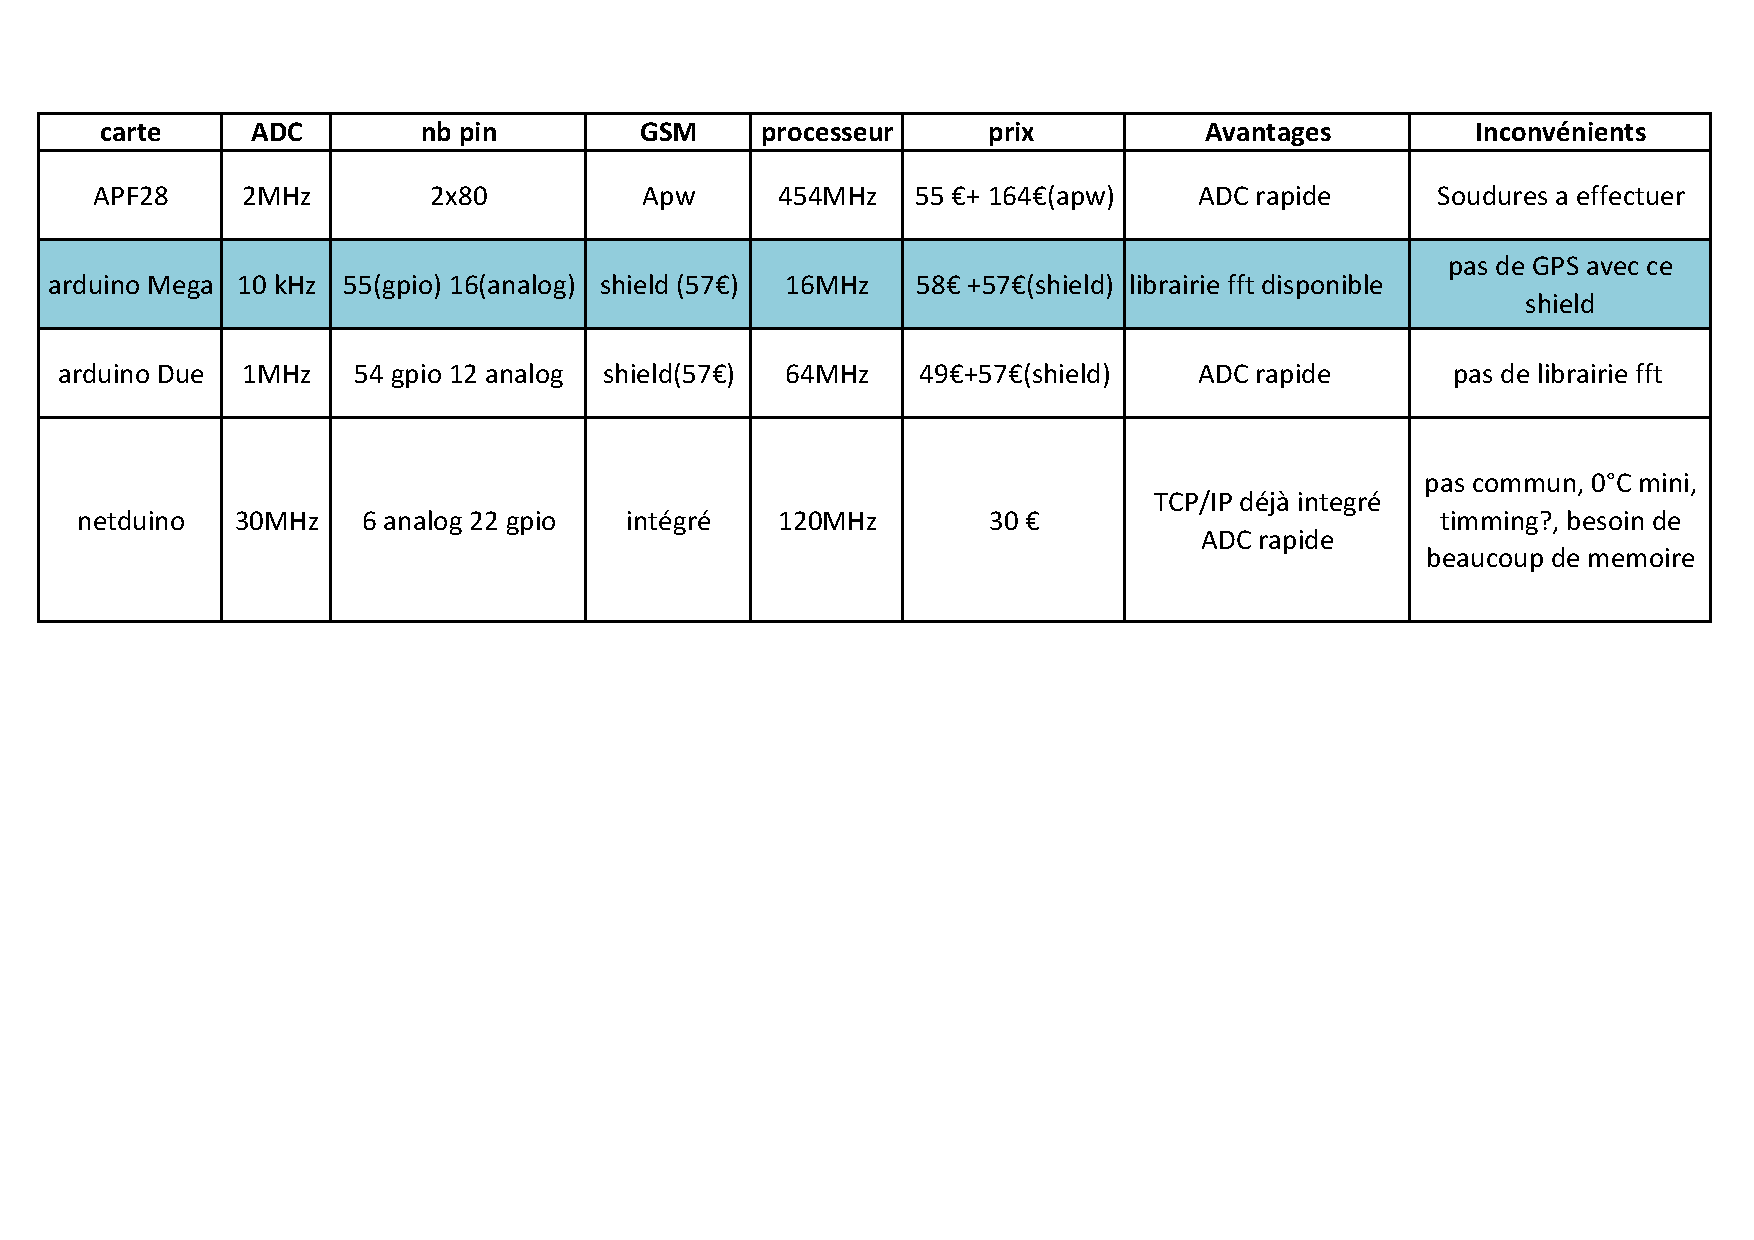
\includegraphics[trim=1cm 11cm 1cm 1cm,scale=0.5]{choixArduino.pdf}
\caption{\label{fig:choixardui} Tableau comparatif des cartes Arduino et équivalents}
\end{figure} 

Nous avons opté pour une carte Arduino Mega 2560, Figure \ref{fig:arduino}, compte tenu de l'existence de nombreuses librairies, notamment pour réaliser une fft, et du prix raisonnable. La carte netduino paraissait également très intéressante, car elle ne nécessite pas de shield supplémentaire pour accéder à internet et était trois fois moins chère que les autres. Cependant, comme ce système est peu utilisé, il sera difficile de trouver de la documentation sur internet. Enfin ce système utilise beaucoup de mémoire pour son fonctionnement, limitant ainsi la capacité de stockage. Nous ne pouvions donc pas envisager cette solution et nous avons donc choisi la carte classique Arduino Mega 2560.


\begin{figure}[h]
\centering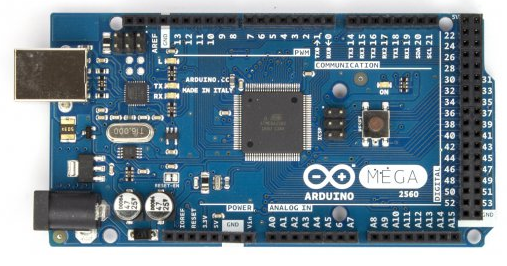
\includegraphics[scale=0.5]{arduino.png}
\caption{\label{fig:arduino} Carte Arduino Mega 2560}
\end{figure} 

\section{Choix de la solution technique}
\vspace{1.5cm}

Nous avons décidé d'opter pour une solution technique simple à déplacer et qui peut ainsi s'adapter à l'utilisateur.
En effet,suite à nos échanges avec notre client, monsieur Singhoff, nous avons remarqué que selon la période de l'année les besoins de l'apiculteur ne sont pas les mêmes. En hivers il veut des informations sur le corps de la ruche alors qu'en été il s'intéresse plus aux hausses qu'il ajoute. Ainsi dans un soucis d'efficacité et de maniabilité, nous voulons intégrer nos capteurs à un cadre en bois que l'apiculteur placera selon ses besoins. Il disposera le cadre sous la partie de la ruche qu'il veut surveiller. Ainsi en hiver, le cadre de mesure sera normalement placé sous la ruche, Figure \ref{fig:rucheBas}, pour vérifier l'activité et les réserves disponibles pour les abeilles. En été, le cadre de mesure sera placé sous une des hausses,comme sur la figure de droite, logiquement la dernière pour suivre la miellée.
\begin{figure}[h]

\begin{minipage}[c]{.46\linewidth}
     \begin{center}
             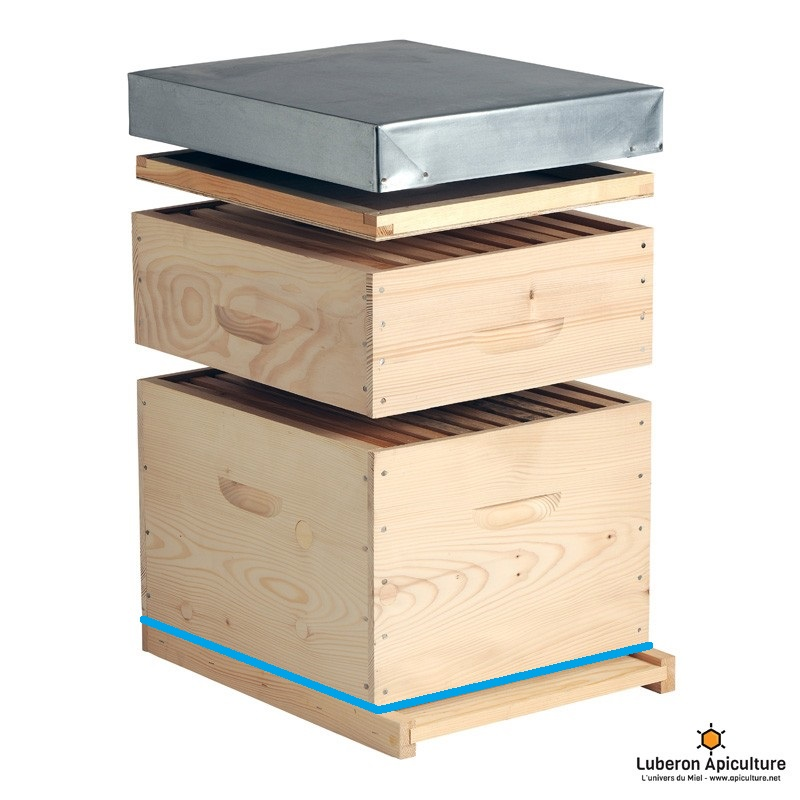
\includegraphics[scale=0.4]{cadreBas.jpg}
             \caption{\label{fig:rucheBas} Position standard du cadre de mesure en hiver}
         \end{center}
   \end{minipage} \hfill
   \begin{minipage}[c]{.46\linewidth}
    \begin{center}
            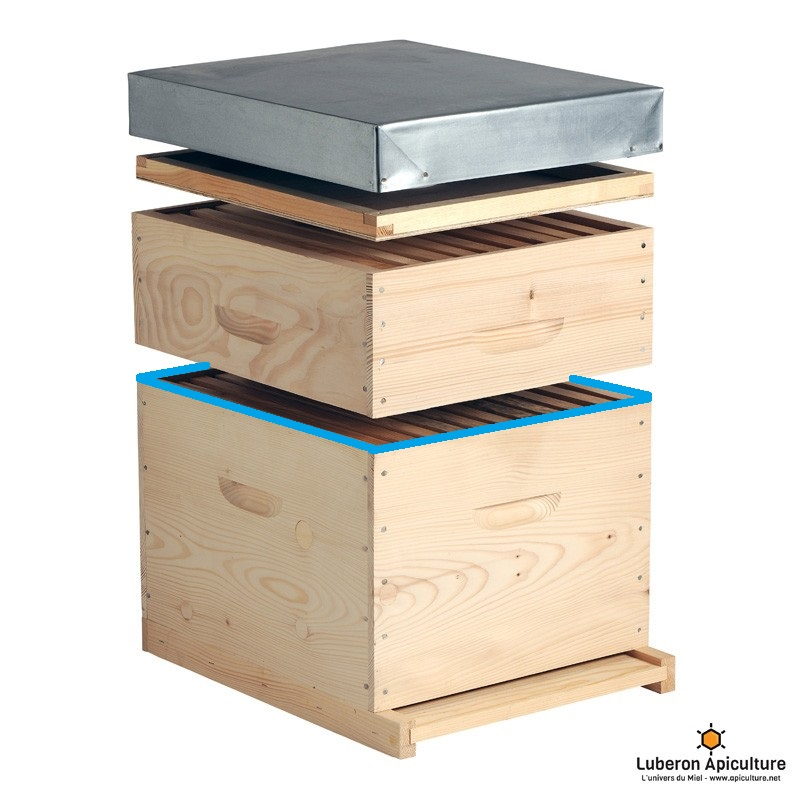
\includegraphics[scale=0.4]{cadreHaut.jpg}
            \caption{\label{fig:rucheBas} Position standard du cadre de mesure en été}
        \end{center}
 \end{minipage}
 \end{figure}

%\chapter{Résultats et analyses}

%analyse des tests et des performances
%analyse des échecs, des décalages et des retards
%Que reste-t-il à faire ? Comment ?


\chapter{Conclusion}

Le projet BMONS a pour ambition de réaliser un système embarqué sur une ruche pour récolter les paramètres physiques de la ruche dans l’optique de détecter les anomalies de comportement des abeilles. Notre équipe s’est donc pencher sur cette problématique avec des notions d’apiculture et de conduite de projet plutôt minces, voici un premier bilan :

Après cette première partie du projet nous pouvons enfin dire que nous comprenons les besoins et les attentes des apiculteurs, par exemple des fonctions auxquelles nous avion pensé, comme la détection du taux d'humidité dans la ruche ne semblent finalement pas primordiale au projet. En revanche des options comme le comptage des abeilles seraient appréciée par les apiculteurs, mais des compromis doivent êtres fait car certaines de ces options entrainent un surcout trop conséquent pour que le projet satisfasse aux exigences initiales.\newline 

Nous devons une grande partie de ces connaissances en apiculture aux réponses précises de M. Franck Singhoff, qui nous a également donné une ruche pour que nous puissions travailler sur l'implémentation des capteurs sur notre prototype. \newline 

Les difficultés que nous avons rencontrées, par exemple lors de la compréhension et de la création des diagrammes nécessaires à l’établissement de la spécification fonctionnelle sur les trois axes, ont été surmontées grâce à l’aide de nos encadrants de projet, mais aussi grâce au dialogue entre les membres du groupe. Le choix des divers composants qui constitueront le prototype a aussi été une source de problèmes, car même si nous avions une idée de quel type de composant nous avions besoin, faire le tri entre tous ceux qui existent nécessite de faire des choix entre par exemple le prix et la précision d’un capteur, et cela influe sur les exigences du projet. \newline

Ces quelques mois de travail en commun nous ont permis d'avoir un aperçu d'ensemble de la conduite d'un projet. Nous nous sommes rendu compte de la quantité de travail que représente la partie ingénierie système sur un projet comme celui-ci. Et bien que nous ne puissions pas prévoir tous les aléas de la seconde partie du projet, ce travail d'anticipation nous permet d'être plus sereins face au travail qu'il reste à fournir.\newline​




\appendix
\part{Annexes}
\chapter{Première annexe}


%\begin{figure}[h!]
%\centering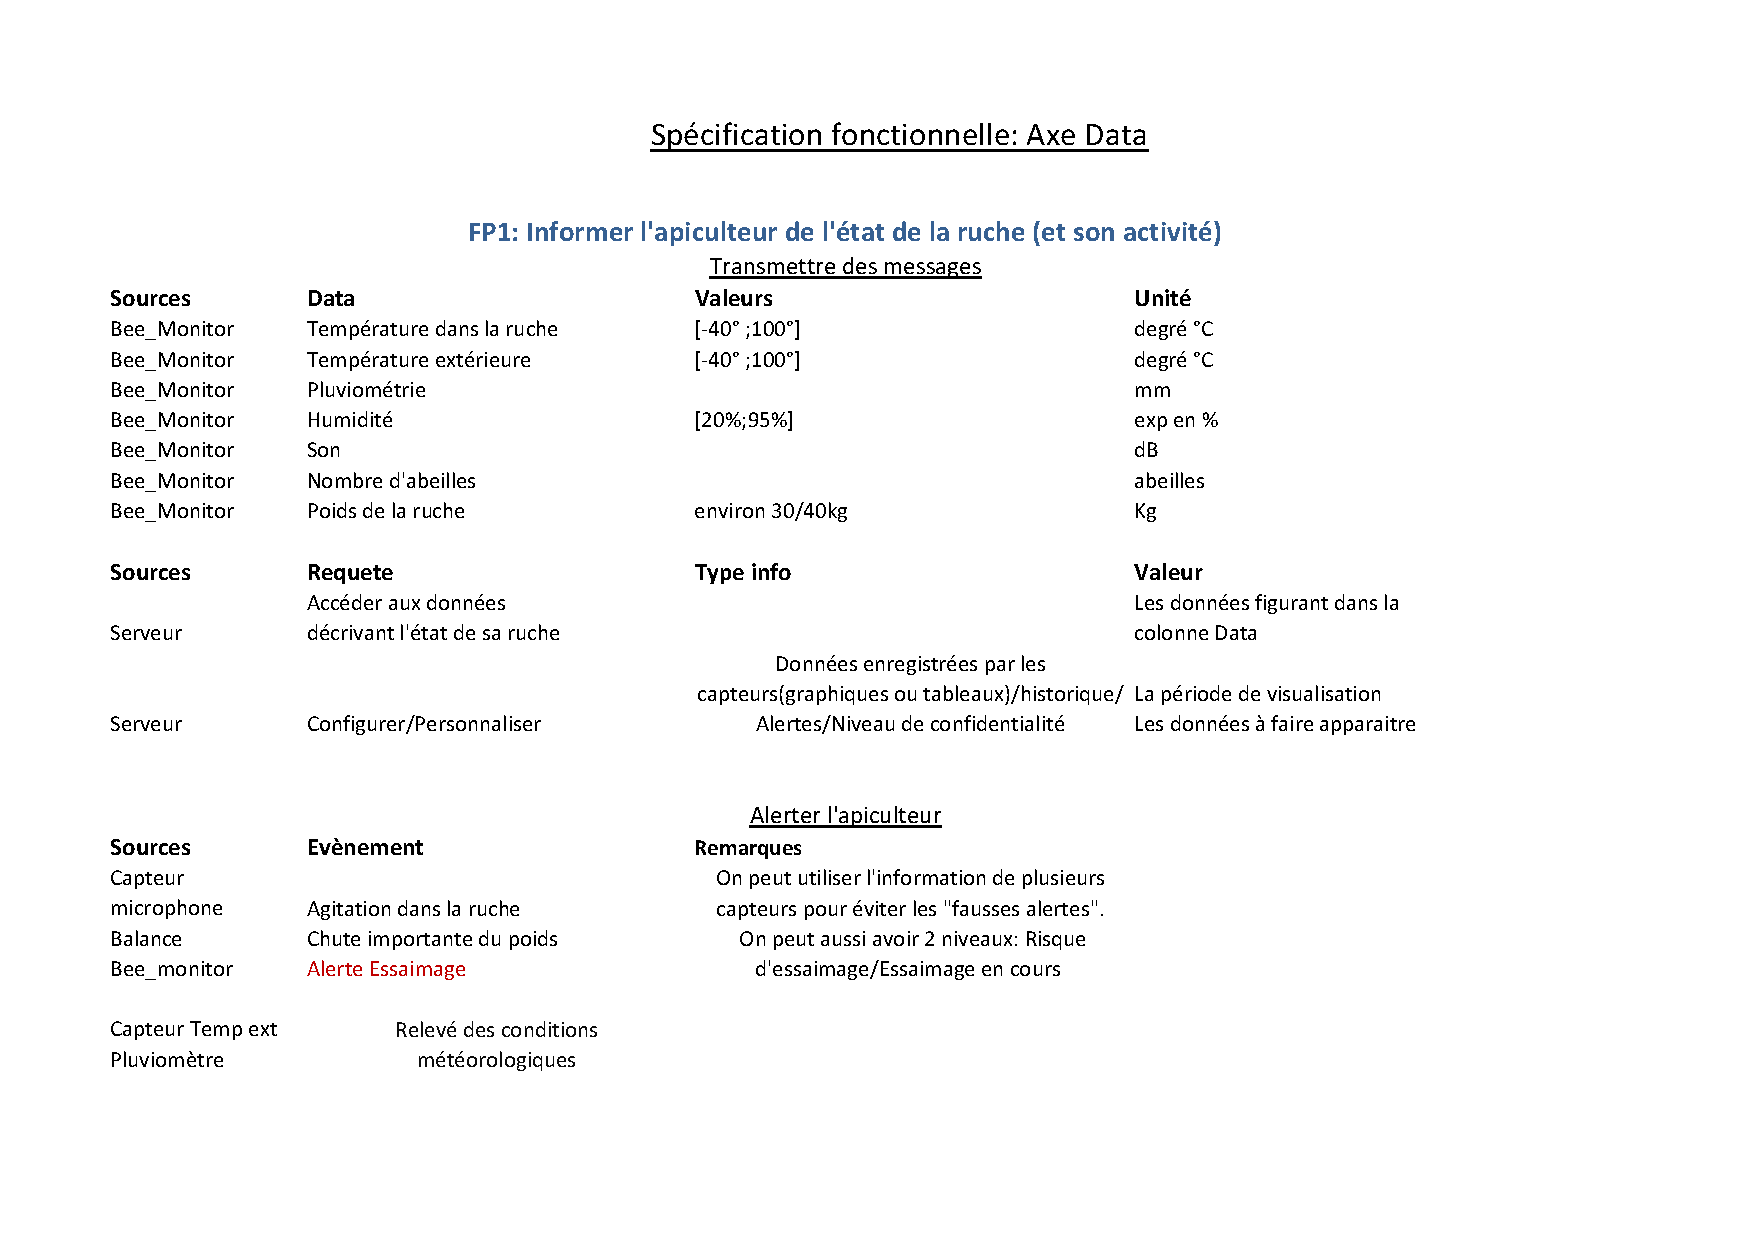
\includegraphics[scale=0.70]{axeData.pdf}
%\end{figure}

\chapter{Deuxième annexe}
\chapter{Troisième annexe}

\backmatter % Partie finale du document, non numérotée

%----------------------------------------------------------------------------------------
%	BIBLIOGRAPHIE
%----------------------------------------------------------------------------------------
\addcontentsline{toc}{part}{Bibliographie}
%\bibliographystyle{apalike-fr}
\bibliographystyle{plain-fr}
\bibliography{bibliographie.bib}
\nocite{*}

%----------------------------------------------------------------------------------------
%	INDEX
%----------------------------------------------------------------------------------------
\cleardoublepage
\phantomsection
\setlength{\columnsep}{0.75cm}
\addcontentsline{toc}{part}{Index}
\label{sec:index}
\printindex

%----------------------------------------------------------------------------------------
%	GLOSSAIRE
%----------------------------------------------------------------------------------------
\cleardoublepage
\phantomsection
\setlength{\columnsep}{0.75cm}
\addcontentsline{toc}{part}{Glossaire}
\printglossaries

%----------------------------------------------------------------------------------------

\end{document}